% !TEX TS-program = XeLaTeX
\documentclass[11pt, twoside]{imsproc}
\usepackage{graphicx}
\usepackage{geometry}
\usepackage{amsmath,amsthm,amssymb,graphicx,tikz,fancyhdr}
\usepackage{booktabs}
\usepackage[colorlinks,citecolor=blue]{hyperref}
\setcounter{page}{1}
\newtheorem{de}{تعریف}[section]
\newtheorem{exa}[de]{مثال}
\newtheorem{alg}[de]{الگوریتم}
\newtheorem{thh}[de]{قضیه}
\geometry{left=2.5cm,right=2.5cm,top=3cm,bottom=3cm,headsep=1.2cm}
\footskip 0.5cm
\usepackage{booktabs}
\usepackage{hyperref}
\newcommand*{\publname}{%
\begin{tabular}{c}
%\includegraphics[width=1.8cm]{UI-logo.pdf}\\
%\url{http://www.ui.ac.ir}
%\vspace{0.2cm}
\end{tabular}
\hfill
\begin{tabular}{c}\toprule
\Large
نسخه‌ی اصلاح شده‌ی مقاله‌ی زیر
%\vspace{0.1cm}
%\scriptsize \bfseries  نشریه ریاضی و جامعه\\
%\vspace{0.1cm}
%\scriptsize
% شاپا (چاپی):--------، شاپا(الکترونیکی): -------- \\
%\vspace{0.1cm}
%\scriptsize
% جلد XX شماره YY (13ZZ)، صص. 1-4\\
%\scriptsize
%\copyright{} 1392 دانشگاه اصفهان 
\\ \bottomrule
\end{tabular}
\hfill
\begin{tabular}{c}
%
\includegraphics[width=2.2cm]{JMS-Logo.png}\\
%\url{http://math-sci.iranjournals.ir}
%\vspace{-0.2cm}
\end{tabular}
}
\usepackage[para*]{manyfoot}
\SetFootnoteHook{\setLTR}
\DeclareNewFootnote[para]{A}
\usepackage{xepersian}
\makeatletter
\let\c@footnoteA\c@footnote
\makeatother
\let\LTRfootnote\footnoteA
\AtBeginDocument{\label{firstpage}}
\AtEndDocument{\label{lastpage}}
\settextfont[Scale=1.1]{XB Niloofar}
\setlatintextfont [Scale=1]{Times New Roman}
\linespread{1.3}
\newsavebox\uilogo
\newsavebox\nologo
\sbox\uilogo{\includegraphics[width=0.8cm]{UI-logo.pdf}}
\sbox\nologo{
\includegraphics[width=1cm]{JMS-Logo.png}}
\makeatletter
\def\seriesno#1{\gdef\@seriesno{#1}}
\def\issueno#1{\gdef\@issueno{#1}}
\def\publicationname#1{\gdef\@publicationname{#1}}
\def\ps@ijheadings{\ps@empty
  \def\@evenhead{%
   \parbox{\textwidth}{%
    \setTrue{runhead}%
    \normalfont\scriptsize
    \usebox\uilogo\hfill
    \def\thanks{\protect\thanks@warning}%
    \leftmark{}{}, \@publicationname/
    جلد
    \@seriesno{}
    شماره
    \@issueno
 (1392) \pageref{lastpage}--\pageref{firstpage}
    \hfill
   \usebox\nologo\vskip0pt
     \vskip-7pt
     \rule{\textwidth}{0.5pt}
      \vskip-12pt
        \rule{\textwidth}{0.5pt}
    }}
  \def\@oddhead{%
   \parbox{\textwidth}{%
    \setTrue{runhead}%
    \normalfont\scriptsize
    \usebox\uilogo\hfill
    \def\thanks{\protect\thanks@warning}%
    \rightmark{}{}, \@publicationname/
    جلد
    \@seriesno{}
    شماره
    \@issueno
 (1392) \pageref{lastpage}--\pageref{firstpage}
    \hfill
   \usebox\nologo\vskip0pt
     \vskip-6pt
     \rule{\textwidth}{0.5pt}
      \vskip-12pt
        \rule{\textwidth}{0.5pt}
    }}
    \def\@evenfoot{\normalfont\small\thepage
     \hfill}
    \def\@oddfoot{\normalfont\small\hfill\thepage}
 }%
\def\enddoc@text{%
\ifx\@empty\@translators \else\@settranslators\fi
  \ifx\@empty\addresses \else\@setaddresses\fi}

\renewcommand*{\@makefnmark}{\hbox{\@textsuperscript{\normalfont\@thefnmark}}}
  \def\MFL@fnotepara#1#2#3{\let\@thefnmark\@empty
    \NCC@makefnmark{\latinfont #2}%
    \MFL@insert#1{\reset@font\footnotesize
      \ifx\@thefnmark\@empty \@tempswafalse \else
        \@tempswatrue
        \protected@edef\@currentlabel{\@thefnmark}%
      \fi
      \color@begingroup
        \if@tempswa
          \setbox\@tempboxa\hbox{\@makefnmark}%
          \ifMFL@paraindent
            \@tempdima.8em \advance\@tempdima-\wd\@tempboxa
            \ifdim \@tempdima<\z@ \@tempdima\z@ \fi
          \else
            \@tempdima\z@
          \fi
        \fi
        \setbox\@tempboxa\hbox{%
          \if@tempswa
            \hskip\@tempdima\unhbox\@tempboxa\nobreak
          \fi
          \ignorespaces\resetlatinfont#3\unskip\strut
          \ifMFL@split \penalty\m@ne\space \else
            \penalty-10 \hskip\footglue
          \fi
        }%
        \dp\@tempboxa\z@ \ht\@tempboxa\MFL@fudgefactor\wd\@tempboxa
        \box\@tempboxa
      \color@endgroup
    }%
  }
\long\def\@footnotetext#1{\insert\footins{%
   \if@RTL@footnote\@RTLtrue\else\@RTLfalse\fi%
    \reset@font\tiny
    \interlinepenalty\interfootnotelinepenalty
    \splittopskip\footnotesep
    \splitmaxdepth \dp\strutbox \floatingpenalty \@MM
    \hsize\columnwidth \@parboxrestore
    \protected@edef\@currentlabel{%
       \csname p@footnote\endcsname\@thefnmark
    }%
    \color@begingroup
      \@makefntext{%
        \rule\z@\footnotesep\ignorespaces\if@RTL@footnote#1\else\latinfont#1\fi\@finalstrut\strutbox}%
    \color@endgroup}}%
%\footdir@temp\footdir@my@ORG@xepersian@footnotetext\@footnotetext{\bidi@footdir@footnote}%
\makeatother

\newcommand{\norm}[1]{\left\lVert#1\right\rVert}

\pagestyle{ijheadings}
\seriesno{1}
\issueno{1}
\publicationname{نشریه ریاضی و جامعه}
\title[
کاربرد بسط تیلور در کاهش حجم
شبکه‌های عصبی پیچشی]
{کاربرد بسط تیلور در کاهش حجم
شبکه‌های عصبی پیچشی برای طبقه‌بندی نقاشی‌های سبک امپرسیونیسم و مینیاتور
}
% مدل‌های یادگیری عمیق}
\author[محمود امین‌طوسی]
{محمود امین‌طوسی}
\date{\today}
\keywords{
شبکه‌های عصبی پیچشی، بسط تیلور، یادگیری عمیق، هرس شبکه،  طبقه‌بندی تصویر}
\thanks{محمود امین‌طوسی\\
تاریخ دریافت: 13yy/xx/xx
\quad
تاریخ پذیرش: 13yy/xx/xx
}
\copyrightinfo{}{(دانشگاه اصفهان)}
%\subjclass[2010]{Analysis; topology}
\makeatletter
\def\ps@firstpage{\ps@plain
\def\@oddfoot{\normalfont\small\hfil\thepage\hfil
\global\topskip\normaltopskip}%
\let\@evenfoot\@oddfoot
\def\@oddhead{\@serieslogo\hss}%
\let\@evenhead\@oddhead % in case an article starts on a left-hand page
}
\makeatother
\begin{document}
\begin{abstract}
بسط تیلور یکی از رو‌ش‌های تقریب توابعی است که از هر مرتبه‌ای مشتق‌پذیر هستند.
روال اصلی یادگیری در شبکه‌های عصبی، مبتنی بر مشتق‌گیری از تابع هدف و استفاده از گرادیان کاهشی برای نیل به پاسخ بهینه است.
 شبکه‌های عصبی پیچشی از مهمترین ابزار حوزه یادگیری عمیق هستند. عمده‌ی این شبکه‌ها متضمن مدل‌هایی با اندازه‌های بزرگ بوده و کاهش حجم این مدل‌ها از موضوعات تحقیقاتی به‌روز می‌باشد. شیوه‌ی اصلی روش‌های کاهش حجم مدل‌ها، هرس کردن اتصالات زائد شبکه‌های عصبی است، که عموماً مبتنی بر اندازه‌ی وزن اتصالات می‌باشند. از جمله‌ی این شیوه‌ها، استفاده از بسط تیلور تابع هدف در محاسبه‌ی اولویت اتصالات، برای حذف آنها از شبکه است. در این نوشتار، این شیوه به صورت مبسوط مورد بررسی قرار گرفته و کاربرد جدیدی از آن در تفکیک تابلوهای نقاشی با سبک‌های امپرسیونیسم (برداشت‌گرایی)‌ و مینیاتور (خُردنگارگری) ارائه شده است. نتایج آزمایش‌ها نشان داده است که با روش مبتنی بر  بسط تیلور می‌توان ۸۳ درصد از اتصالات شبکه را انتخاب و حذف نمود، بدون آنکه دقت مدل در این کاربرد خاص کاهش پیدا کند.
\end{abstract}
\maketitle
\vspace*{-5mm}
\section{مقدمه}


مدل‌های یادگیری عمیق%
\LTRfootnote{Deep Learning}
در سالیان اخیر
  کارایی فوق‌العاده‌ای در شناسایی اشیاء به نمایش گذاشته‌اند
\cite{DLSurvey2019Jiao}.
روشهای
\lr{RCNN} \cite{RCNN}،
\lr{Mask R-CNN} \cite{MaskRCNN2020He}
و
\lr{YOLO} \cite{redmon2017yolo9000}
از جمله تحقیقات پر ارجاع و کارا در این حوزه هستند.
شبکه‌های عصبی پیچشی%
\LTRfootnote{Convolutional Neural Networks (CNNs/ConvNets)}
یکی از ابزارهای اصلی مورد استفاده در این زمينه است که در این تحقیقات به‌کار گرفته شده‌اند.
این شبکه‌ها را می‌توان توسیعی از شبکه‌های عصبی مرسوم از نوع پرسپترون چند لایه%
\LTRfootnote{Multi Layer Perceptron}
دانست که عمل پیچش%
\LTRfootnote{Convolution}
  یا فیلتر کردن تصاویر را برای استخراج ویژگی‌های مفید انجام می‌دهند و معمولاً متضمن هزاران نورون و میلیو‌نها اتصال هستند.
داشتن مجموعه دادگان بزرگ از الزامات مدلهای پیچیده‌ی جدید این حوزه است.
این مجموعه داده‌ها یا به صورت مستقیم در خود مدل استفاده می‌شود و یا در ایجاد معماری‌هایی مانند
\lr{VGG} \cite{VGG_Simonyan15}،
\lr{ResNet} \cite{ResNet_He_2016_CVPR}،
\lr{AlexNet} \cite{NIPS2012_4824} %60 M parameters
و
\lr{DarkNet}\LTRfootnote{\url{https://pjreddie.com/darknet/}} \cite{redmon2017yolo9000}
 به‌کار برده شده‌اند، که مبنای بیشتر مدل‌های مرتبط است.
 هر یک از این مدل‌ها تفاوت‌هایی از منظر تعداد نورون‌ها، نحوه‌ی اتصالات و نوع لایه‌های شبکه با هم دارند.
  اندازه این مدل‌ها معمولاً بسیار بزرگ بوده و شامل میلیون‌ها پارامتر هستند.
% به این مدل‌ها
%\textit{
%مدل از قبل آموزش دیده
%}
%اطلاق می‌شود.
شکل
\ref{fig:vgg16}
ساختار مدل
\lr{VGG16}
را نشان می‌دهد که بالغ بر ۱۳۰ میلیون پارامتر دارد.
%
در روال یادگیری یک شبکه عصبی،‌ در واقع وزن اتصالات هستند که باید به نحوی تنظیم شوند که عمل خواسته شده انجام شود. حجم یک مدل متناسب با تعداد نورون‌ها و اتصالات آن می‌باشد که جزء پارامترهای مدل می‌باشند.%
%\footnote{ در این نوشتار پارامترها، وزن‌‌ها و اتصالات معادل هم درنظر گرفته شده‌اند.
% }.

   برای آموزش چنین مدل‌هایی، حجم زیاد داده و توان پردازشی بالا
% به مانند
%\lr{GPU}
%ها
 مورد نیاز است.
کاهش حجم این مدل‌ها که از طریق حذف تعدادی از نورون‌ها و اتصالات آنها یا حذف برخی از اتصالات انجام می‌شود، از موضوعات مورد علاقه محققین یادگیری عمیق است.
هرس و کاهش اندازه‌ی مدل می‌تواند حجم یک مدل اولیه‌ی مثلاً 500 مگابایتی را به 50 مگابایت کاهش دهد، که برای استفاده در یک برنامه‌ی اندرویدی مناسب‌تر است.
روش‌های مختلفی برای کاهش تعداد نورون‌ها یا تعداد اتصالات شبکه‌ها ارائه شده است.
اولین بار ایده دراپ‌اوت%
\LTRfootnote{Dropout}
توسط هینتون%
\footnote{
جفری هینتون
\lr{(Geoffrey Hinton)}
روانشناس شناختی، دانشمند علوم کامپیوتر و یکی از افرادی است که از آنها به عنوان پدران یادگیری عمیق یاد می‌شود.
}
  و همکاران
\cite{Hinton2012dropout}
  برای شبکه‌های عصبی مطرح شد؛ در این شیوه نورون‌هایی از شبکه به صورت تصادفی  حذف می‌شوند.
% Who Is the Father of Deep Learning?
% https://ieeexplore.ieee.org/document/9070967
    گرچه ایده‌ی اصلی ساده است اما در عمل کارایی بسیار خوبی داشته و عموم مدل‌های جدید، متضمن چندین لایه دراپ‌اوت هستند.
ایده‌ی دراپ‌اوتِ هینتون توسط وان
\LTRfootnote{L.~Wan}
  و همکاران
\cite{pmlr-v28-wan13}
به حذف تصادفی وزن‌ها تعمیم داده شد و بعداً
کارایی این شیوه بر روی شبکه‌های پیچشی مورد بررسی قرار گرفت
\cite{WU20151}.
شیوه‌ی کلی دیگری که در هرس وزن‌های شبکه‌ها استفاده می‌شود، منظم‌سازی%
\LTRfootnote{Regularization}
است که توسط محققین مختلف
 در قالب یک مسئله‌ی بهینه‌سازی تُنُک%
\LTRfootnote{Sparse Optimization}
فرموله و حل شده است
\cite{conf/cvpr/LiuWFTP15,
DBLP:journals/corr/abs-1802-10280,
NIPS2016_6504,mitsuno2020hierarchical}؛
تابع هدف مسئله‌ی بهینه‌سازی مدنظر در بخش
\ref{sec:model_size_reduction}
آمده است.
%از روش‌های منظم‌سازی برای حل مسئله استفاده شده است.
در این شیوه‌ها عموماً
نُرم صفر وزن‌های اتصالات شبکه به عنوان جمله‌ی منظم‌ساز، به تابع هدف مسئله افزوده می‌شود. نُرم صفر یک بردار، تعداد عناصر غیرصفر آن است.
%و روال بهینه‌سازی همزمان با کمینه کردن تابع هدف به کاهش نُرم وزن‌ها نیز می‌پردازد.
 وزن‌های با مقادیر کوچکِ نزدیک به صفر، هرس شده و حجم مدل کاهش می‌یابد.
مولچانوف%
\LTRfootnote{P.~Molchanov}
و همکاران از پژوهشگران شرکت ان‌وی‌دیا%
\LTRfootnote{Nvidia}%, \url{https://www.nvidia.com/}}
یک شیوه‌ی مبتنی بر استفاده از بسط تیلور تابع هدف ارائه و برتری آن را نسبت به چندین روش مرسوم در این حوزه نشان داده‌اند
\cite{MolchanovTKAK17}.

\begin{figure*}[t]
\centering
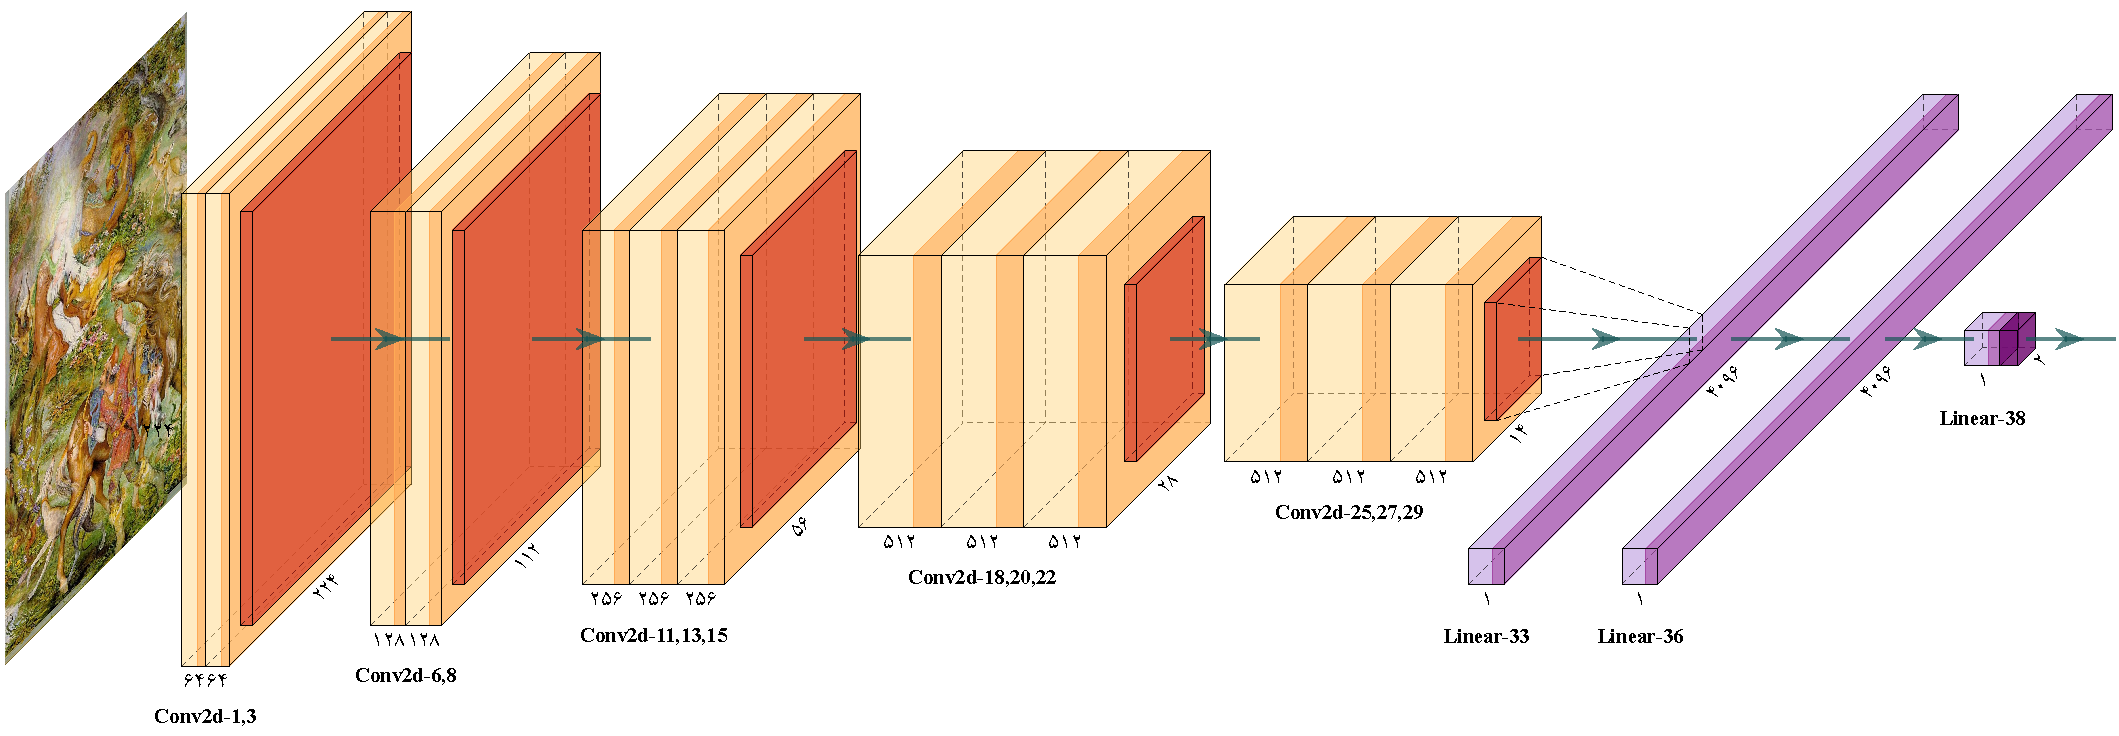
\includegraphics[width=1\linewidth]{images/vgg16.pdf}
\caption{
معماری مدل
\lr{VGG16} \cite{VGG_Simonyan15}
با بیش از ۱۳۰ میلیون پارامتر (وزن). ورودی شبکه، یک تصویر و خروجی آن مشخص‌کننده‌ی طبقه‌ی تصویر ورودی است.
% به دلیل حجم زیاد تعداد پارامترها، فقط ساختار لایه‌های شبکه و اندازه تقریبی خروجی هر لایه نمایش داده می‌شود. % هدف این نوشتار کاهش تعداد وزن‌های این مدل،‌به نحوی است که همچنان کارایی اولیه‌ی خود را حفظ کند. توضیحات بیشتر درخصوص این مدل در بخش
%\ref{sec:NN}
%  آمده است.
}
\label{fig:vgg16}
\end{figure*}


هدف این نوشتار، مقایسه‌ی این روش‌ها نیست؛ بلکه هدف اصلی، بیان چگونگی روش کار مولچانوف و همکاران
~\cite{MolchanovTKAK17}
است که در آن از بسط تیلور برای هرس اتصالات شبکه استفاده شده است. در مقاله‌ی مذکور، شیوه‌ی مورد استفاده به اختصار بیان شده است؛ در این نوشتار این روش به تفصیل بیان شده و در ضمنِ یک کاربرد جدید،‌ کارایی آن نشان داده شده است.
به عنوان کاربردی جدید، مسئله‌‌ی تفکیک دو سبک نقاشی امپرسیونیسم%
\LTRfootnote{Impersionism}
 (برداشت‌گرایی) و
مینیاتورهای ایرانی با سبک محمود فرشچیان در نظر گرفته شده است که در بخش
\ref{sec:results}
 بیان می‌شود.

% چارچوب مقاله در ادامه نوشتار به ترتیب زیر خواهد بود.
 از آنجا که برای بیان مسئله، یک نگرش مقدماتی بر شبکه‌های عصبی پیچشی لازم است، در بخش
 \ref{sec:NN}، 
 به مرور کوتاهی بر شبکه‌های عصبی پرداخته شده است. مدل ساده پرسپترون، که سنگ بنای شبکه‌های عصبی است، نحوه‌ی آموزش آن و مدل‌های شبکه‌های عصبی پیچشی در این بخش بیان شده‌اند.
 در بخش
 \ref{sec:model_size_reduction}، 
به معضل حذف اتصالات اضافی در شبکه‌های عصبی پیچشی،
  بسط تیلور و چگونگی استفاده از آن در روال حذف اتصالات زائد پرداخته شده است.
 در بخش~\ref{sec:results}، 
مسئله‌ی تفکیک سبک‌های نقاشی به عنوان کاربردی جدید از شبکه‌های عصبی پیچشی عنوان شده و نتایج استفاده از شیوه‌ی مبتنی بر بسط تیلور برای کاهش حجم مدل مورد استفاده ذکر شده است.
 نتایج آزمایش‌های انجام شده نشان داده است که با شیوه‌ی مورد بحث، می‌توان در عین حفظ دقت مدل اصلی،  ۸۳ درصد از اتصالات شبکه را حذف کرد.
  آخرین بخش به جمع‌بندی اختصاص یافته است.


\section{مروری بر شبکه‌های عصبی}\label{sec:NN}
مدل‌های شبکه‌‌های عصبی مصنوعی، سال‌ها به امید ایجاد عملکردی مشابه مغز انسان در موضوعاتی نظیر تشخیص صحبت و تصویر در شاخه‌های هوش مصنوعی مورد مطالعه قرار گرفته‌اند. ساختار این مدل‌ها که الهام‌گرفته از شبکه‌های عصبی زیستی است، متشکل از تعدادی عنصر محاسباتی (نورون‌ها، گره‌ها، نودها) است که از طریق وزن‌هایی تطبیقی%
\LTRfootnote{Adaptive Weights}
  به هم متصل شده و به موازات یکدیگر کار می‌کنند. ساده‌ترین ساختار گره، معمولاً به صورت غیرخطی است که در آن، هر کدام از ورودی‌ها در وزن خاصی ضرب شده و حاصل‌جمع آنها پس از عبور از یک تابع، خروجی را به دست می‌آورد (شکل
  \ref{fig:perceptron}).
   هر شبکه‌ی عصبی، علاوه بر معماری (توپولوژی) شبکه و مشخصات گره یا نود (یعنی نوع تابع آن، موسوم به تابع فعالیت%
\LTRfootnote{Activation Functions})،
 دارای یک روال یادگیری یا آموزشی نیز می‌باشد. عمل یادگیری%
 \LTRfootnote{Training or Learning Rule}
   در شبکه‌های عصبی، به معنی تنظیم درست وزن‌ها است به گونه‌ای که شبکه با ورود داده‌های مشخص، پاسخ مورد انتظار را تولید کند. %قاعده‌ی یادگیری
%    مشخص می‌کند که در هنگام آموزش شبکه، وزن‌ها چطور باید بهنگام شوند تا شبکه وابسته به مقدار ورودی داده شده، خروجی مورد انتظار را تولید کند.
    % آموزش شبکه، برای بالابردن دقت و درستی تشخیص است.
     روش‌های طراحی شبکه و قواعد آموزش آن، موضوع بسیاری از تحقیقات گذشته و اکنون است. با دسترسی به داده‌های آموزشی حجیم و افزایش تعداد نودها و اتصالات، تنظیم وزن اتصالات بسیار زمان‌بر و نیازمند توان پردازشی زیاد است. ظهور کارت‌های گرافیکی قدرتمند در کنار ابداع روش‌های بهتر بهینه‌سازی و انواع جدیدتر توابع فعالیت، باعث اوج‌گیری مجدد شبکه‌های عصبی در قالب یادگیری عمیق%
\LTRfootnote{Deep Learning}
       شده است.
%مدلهای شبکه‌های عصبی مصنوعی،  سالها به امید ایجاد عملکردی مشابه مغز انسان در موضوعاتی نظیر تشخیص صحبت و تصویر مورد مطالعه قرار گرفته‌اند. این مدل‌ها از تعدادی عنصر محاسباتی غیرخطی%
%\LTRfootnote{Nonlinear Computational Element}
% تشکیل شده‌اند که به موازات یکدیگر کار می‌کنند.
% % شبکه‌های  عصبی زیستی است.
%  این عناصر محاسباتی (نورون‌ها، گره‌ها یا نودها)
% از طریق وزن‌هایی%
%\LTRfootnote{Weights}
%تطبیقی%
%\LTRfootnote{Adaptive}
%% که معمولا برای افزایش کارایی شبکه در هنگام استفاده تغییر می‌کنند،
% به هم متصل شده‌‌اند. عمل یادگیری در شبکه‌های عصبی به معنی تنظیم درست این وزن‌هاست، به گونه‌ای که شبکه در قبال ورود داده‌های مشخص، خروجی مورد انتظار را بدست دهد.
%%یک مدل شبکه‌های عصبی می‌تواند یک نورون و دو وزن داشته باشد یا هزاران نورون و چندین میلیون اتصال داشته باشد.
%%مدل‌های شبکه‌های عصبی  پردازش مدنظر را از طریق عناصر محاسباتی که با رابط‌‌‌‌هایی با وزن‌های مختلف به یکدیگر متصل شده‌اند، انجام می‌دهند.
%عناصر محاسباتی یا گره‌های مورد استفاده در مدل‌های شبکه‌های عصبی، معمولاً غیر خطی هستند. ساده ترین گره،
%%$n$
%  ورودی‌های خود را که هر کدام در وزن خاصی ضرب شده‌اند، جمع بسته،  حاصل را از یک تابع (عموماً)‌ غیر خطی
%%\LTRfootnote{nonlinearity}
%  عبور می‌دهد (شکل
%\ref{fig:perceptron}).
%  هر مدلِ شبکه‌های عصبی، با معماری (توپولوژی) شبکه، مشخصات گره یا نود %(آستانه و نوع تابع فعالیت آن)
%   و قاعده‌ی آموزش یا یادگیری%
%\LTRfootnote{Training or Learning Rule}
%مشخص می‌شود.
%این قواعد مجموعه‌ای از وزن‌ها را تعیین و مشخص می‌کند که وزن‌ها چطور باید در هنگام آموزش شبکه بهنگام شوند. روش‌های طراحی شبکه و قواعد  آموزش آن موضوع بسیاری از تحقیقات بوده و هست.
%  با افزایش تعداد نودها و اتصالات، آموزش شبکه (تنظیم وزن‌های اتصالات) نیازمند زمان اجرای زیاد و توان پردازشی بالایی خواهد بود.
%دسترسی به داده‌های آموزشی حجیم و قابلیت‌های پردازشی زیاد، مانند کارت‌های گرافیکی در کنار ابداع روش‌های بهتر بهینه‌سازی و انواع جدیدتر توابع فعالیت%
%\LTRfootnote{Activation Functions}
%باعث اوج‌گیری مجدد توجه به شبکه‌های عصبی در قالب یادگیری عمیق%
%\LTRfootnote{Deep Learning}
%شده است.

%  اساس فرآیند یادگیری در شبکه‌های عصبی بر تنظیم درست وزن‌های شبکه استوار است؛ به نحوی که شبکه بتواند وظیفه مدنظر را به خوبی اجرا کند.
  یکی از ابزارهای حوزه یادگیری عمیق، شبکه‌های عصبی پیچشی%
\LTRfootnote{Convolutional Neural Networks}
    است که با دقت زیاد قادر به تفکیک نمونه‌ها در قالب دسته‌های از پیش مشخص است. مثال مشهوری که امروزه در حوزه یادگیری عمیق استفاده می‌شود، دسته‌بندی تصاویر سگ و گربه است. با استفاده از صدها تصویر متفاوت سگ و گربه، یک شبکه عصبی پیچشی آموزش می‌بیند تا مشخص کند که یک تصویر جدید (سگ یا گربه) متعلق به کدام دسته است. روال یادگیری در بسیاری از انواع شبکه‌ها از~جمله شبکه‌های عصبی پیچشی، بر پایه‌ی مدل پرسپترون%
\LTRfootnote{Perceptron}
      است. در ادامه، مدل پرسپترون و شبکه‌های عصبی پیچشی به صورت مختصر بیان می‌شوند.

%یکی از کاربردهای اصلی شبکه‌های عصبی، طبقه‌بندی نمونه‌ها به رده‌های از پیش مشخص است.  مثال مشهوری که امروزه در حوزه یادگیری عمیق استفاده می‌شود دسته‌بندی کننده تصاویر سگ و گربه است. با استفاده از صدها تصویر متفاوت سگ‌ و گربه‌، یک شبکه عصبی پیچشی%
%\LTRfootnote{Convolutional Neural Networks}
%آموزش می‌بیند که با دقت بسیار زیاد قادر به تفکیک تصاویر جدید است و می‌تواند مشخص کند تصویر جدید (سگ یا گربه) متعلق به کدام دسته است.
%پرسپترون تک لایه%
%\LTRfootnote{Single Layer Perceptron}،
% ساده‌ترین مدل شبکه عصبی است.
%با نظارت
%\LTRfootnote{Supervised}
%  می‌باشد.
%  چارچوب کلی یادگیری در این مدل، پایه‌ی روال آموزش در شبکه‌های عصبی و منجمله شبکه‌های عصبی پیچشی است.
%لذا در ادامه ابتدا مروری خواهیم داشت بر مدل پرسپترون و سپس شبکه‌های عصبی پیچشی به صورت مختصر بیان خواهند شد.

\subsection{مدل پرسپترون}

%\begin{figure}[t]
%\centering
%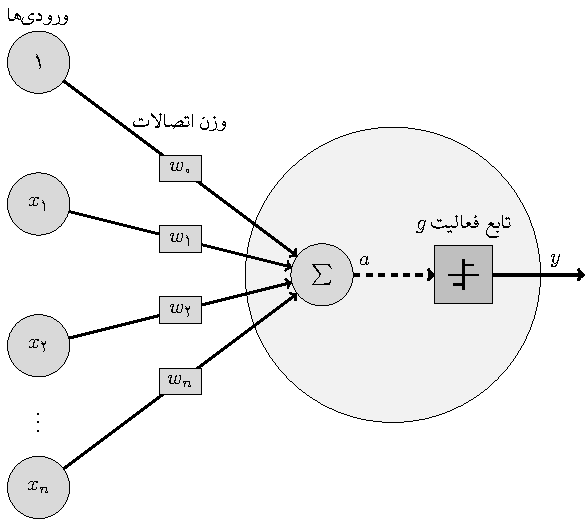
\includegraphics[width=.8\linewidth]{images/perceptron_01}
%\caption{مدل پرسپترون}
%\label{fig:perceptron}
%\end{figure}


% Perceptron05
%\begin{equation}
%\label{output}
%output =
%\begin{cases}
%+1 & \text{for} \sum_{i = 1}^n w_i x^{(s)}_i > 0\\
%-1 & \text{for} \sum_{i = 1}^n w_i x^{(s)}_i \leq 0,
%\end{cases}
%\end{equation}
%
%\begin{equation}
%w_i^{\rm new} =  w_i^{\rm old} + r (O^{(s)} - output) x^{(s)}_i,
%\label{learn}
%\end{equation}

روال اصلی یادگیری در شبکه‌های پرسپترونی مبتنی بر
 کمینه کردن
 % تابع هدف است. انواع مختلفی از  تابع هدف موجود هستند که پایه‌ی همه‌ی آنها کم کردن
 خطای شبکه است. اگر هدف شبکه، طبقه‌بندی باشد، تابع هدف می‌تواند کاهش تعداد نمونه‌هایی باشد که به صورت نادرست دسته‌بندی شده‌اند%
\LTRfootnote{Miss-Classification Error}.
فرض کنید که مسئله‌ی موردنظر،‌ طبقه‌بندی داده‌ها به دو کلاس است که برچسب دو کلاس (طبقه) به ترتیب صفر و یک درنظر گرفته شده و خروجی شبکه، صفر یا یک است.
اگر
$y_i$%
\LTRfootnote{Target}
برچسب درست طبقه‌ی نمونه‌ی $i$ام و
$\hat{y}_i$
خروجی شبکه برای این نمونه باشد، مجموع زیر بیانگر تعداد نمونه‌هایی است که
به اشتباه طبقه‌بندی شده‌اند:
\begin{equation}
\sum_{i}|y_i-\hat{y}_i|
\label{eq:missClassification}
\end{equation}
%تابع هدف بر حسب وزن‌های شبکه است. برای نمایش وابستگی تابع خطا به وزن‌های شبکه اجزای شبکه را به صورت مجزا نام‌گذاری می‌کنیم.
يعنی 
$\hat{y}_i$
که خروجی شبکه‌ی عصبی است ممکن است منطبق بر مقدار مورد انتظارِ
$y_i$
 باشد (طبقه‌بندی درست) یا نباشد (طبقه‌بندی نادرست). نحوه‌ی محاسبه‌ی خروجی شبکه عصبی، در ادامه آمده است. 

\begin{figure}[t]
    \centering
    \begin{minipage}{.3\textwidth}
        \centering
			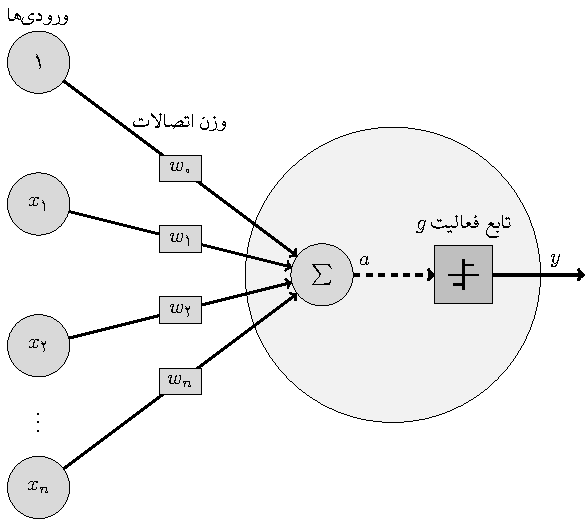
\includegraphics[width=1\linewidth]{images/perceptron_01}
			\caption{مدل پرسپترون}
			\label{fig:perceptron}
    \end{minipage}%
    \hfill
    \begin{minipage}{.28\textwidth}
        \centering
			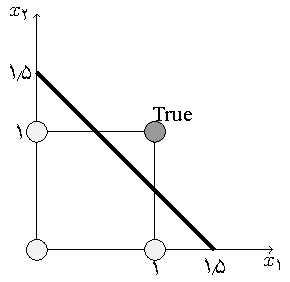
\includegraphics[width=1\linewidth]{images/OR-plot}
			\caption{ترکیب عطفی $x_1$ و $x_2$.
بالای	خط پررنگ، ناحیه‌ای است که
$x_1 \wedge x_2$،
\lr{True}
است.}
			\label{fig:OR-plot}
	\end{minipage}
	\hfill
    \begin{minipage}{0.33\textwidth}
        \centering
			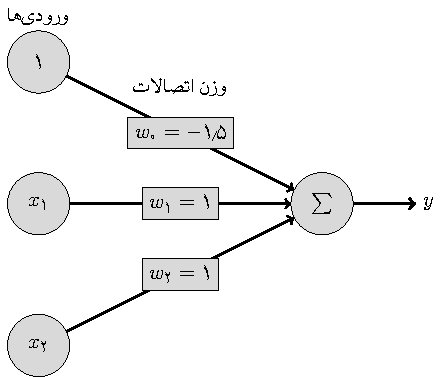
\includegraphics[width=1\linewidth]{images/perceptron_or}
			\caption{مدل پرسپترون برای ترکیب عطفی $x_1$ و $x_2$؛
نمایش‌دهنده‌ی خط جداساز شکل 
\ref{fig:OR-plot}
است.}
			\label{fig:perceptron_or}
    \end{minipage}
\end{figure}

همان‌گونه که در ابتدای بخش اشاره شد یک نود در شبکه‌های عصبی مصنوعی، سیگنالهای ورودی را از $n$‌ نورون دیگر یا ورودی‌های شبکه دریافت کرده و مجموع وزن‌دار این سیگنال‌ها، ورودی تابع فعالیت
%\LTRfootnote{Activation function or Logistic function}
  نورون را شکل می‌دهد (شکل
\ref{fig:perceptron}).
  یک مدل ساده با تابع فعالیت همانی، در واقع مشخص‌کننده‌ی یک مرز خطی برای دو ناحیه در صفحه است که هر ناحیه، یک دسته را مشخص می‌کند. با یک مثال، نحوه‌ی پیاده‌سازی ترکیب عطفی
  $x_1$
  و
  $x_2$
با مدل پرسپترون را نشان خواهیم داد.
خط
$w_0+w_1x_1+w_2x_2=0$
با
$w_0=-1.5$
و
$w_1=w_2=1$
را درنظر بگیرید (خط پررنگ در شکل
 \ref{fig:OR-plot}).
  با این فرض که
\lr{True}
و
\lr{False}
به ترتیب با یک و صفر نشان داده شوند، خط فوق، مشخص‌کننده‌ی مرز تصمیم‌گیری برای
$x_1 \wedge x_2$
 است.
اگر
$x_1$
و
$x_2$
هر دو یک
\lr{(True)}
  باشند،
$x_1+x_2-1.5$،
مثبت و در سه حالت دیگر، منفی خواهد شد. اگر مثبت و منفی را به ترتیب متناظر با
\lr{True}
و
\lr{False}
 فرض کنیم، خط فوق عمل ترکیب عطفی دو ورودی خود را انجام می‌دهد.
 مدل پرسپترون نمایش داده شده در شکل
 \ref{fig:perceptron_or}، 
 حاصل 
 $w_0+w_1x_1+w_2x_2$
 را برای 
 $x_1$
 و
 $x_2$
ورودی محاسبه می‌کند که با توضیح داده شده،‌ در واقع عمل ترکیب عطفی ورودی‌های خود را انجام می‌دهد. 
%از دیدگاه طبقه‌بندی 
%  اگر داده‌ها فقط یک مؤلفه‌ی $x$ داشته باشند، معادله خط جداساز صفحه به صورت $y=wx+b$ است. در ساده‌ترین حالت، تشخیص طبقه‌ی ورودی داده شده، با قرار دادن نقطه جدید در معادله‌ی خط و بررسی مثبت یا منفی بودن $y$ صورت می‌پذیرد. هر یک از وضعیت‌های مثبت و منفی یکی از دو طبقه (کلاس) مورد بررسی را مشخص می‌کنند.
  % همان‌گونه که قبلاً اشاره شد این واحدهای کوچک محاسباتی عموماً غیرخطی هستند،
   %مجموع محاسبه شده در معادله‌ی خط (ابرصفحه در فضای چند بعدی) از تابع فعالیت عبور داده می‌شود.
معادله‌ی ساده‌ی خط فوق که در اینجا مشخص‌کننده‌ی یک مرز خطی بود، در فضاهای با ابعاد بالاتر (تعداد مؤلفه‌ها یا تعداد ویژگی‌های بیشتر) یک ابرصفحه‌ی جداساز را مشخص می‌کنند.
    فرض کنید مطابق رابطه‌ی زیر،
%\eqref{eq:noronIn}،
    $a$
     مجموع وزن‌دار ورودی‌های نورون باشد:
  \begin{equation}
  \label{eq:noronIn}
  a=\sum_{j=1}^n w_j x_j+b
\end{equation}
که در آن
$n$
تعداد ویژگی‌ها (مؤلفه‌ها)ی هر نمونه،
    $b$
عرض از مبدأ (بایاس)،
 $x_j$،
$j$امین
سیگنال ورودی و
$w_j$
وزن اتصال ورودی $j$ام به این نورون است.
برای راحتی، عموماً یک ورودی
 $x_0=1$
 درنظر گرفته شده و
$w_0=b$
به عنوان وزن اتصال این ورودی منظور می‌شود. به این ترتیب، رابطه بالا به صورت زیر نوشته می‌شود:
\begin{equation}
  a=\sum_{j=1}^n w_j x_j+b=\sum_{j=0}^n w_j x_j=\mathbf{w}^T{\mathbf{x}}
\end{equation}
که در آن، 
    ${\mathbf{x}}=[x_0=1,x_1,\cdots,x_n]^T$
بردار ورودی و
      $\mathbf{w}=[w_0=b,,w_1,\cdots,w_n]^T$
وزن اتصالات می‌باشد.
سیگنال خروجی
$\hat{y}$
یا پاسخ نورون،‌ تابعی از ورودی آن است:
\begin{equation} 	
  \hat{y}=g(a)=g\left(\sum_{j=0}^n w_j x_j\right)=g(\mathbf{w}^T{\mathbf{x}})
\end{equation}
تابع $g(.)$ تابع فعالیت نامیده می‌شود. توابع مختلفی به عنوان تابع فعالیت درنظر گرفته می‌شوند که تابع سیگمویید با ضابطه‌ی
$g(x)=\frac{1}{1+e^{-x}}$
از مرسوم‌ترین آنهاست.
این ساختار ساده «مدل پرسپترون» نامیده می‌شود که در
شکل
\ref{fig:perceptron}
نشان داده شده است.

%\begin{figure}[t]
%\centering
%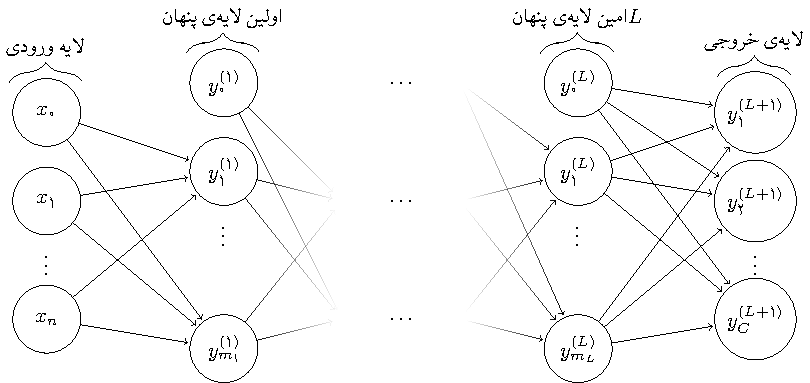
\includegraphics[width=1\linewidth]{images/MLP}
%\caption{شبکه عصبی پرسپترون چند لایه}
%\label{fig:MLP}
%\end{figure}

\begin{figure}[t]
    \centering
%    \begin{minipage}{.4\textwidth}
%        \centering
%			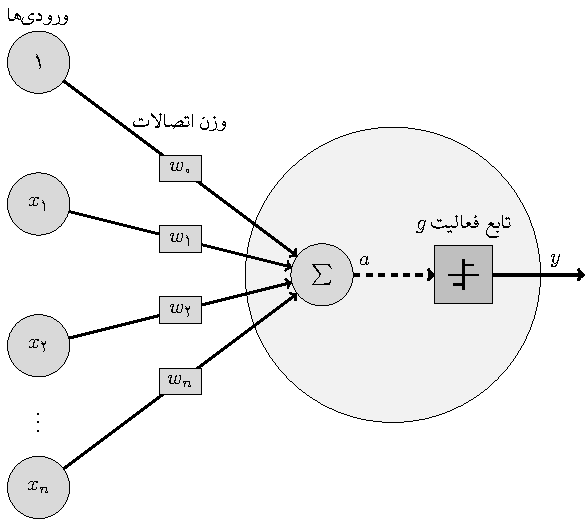
\includegraphics[width=.8\linewidth]{images/perceptron_01}
%			\caption{مدل پرسپترون}
%			\label{fig:perceptron}
%    \end{minipage}%
%    \begin{minipage}{0.6\textwidth}
        \centering
			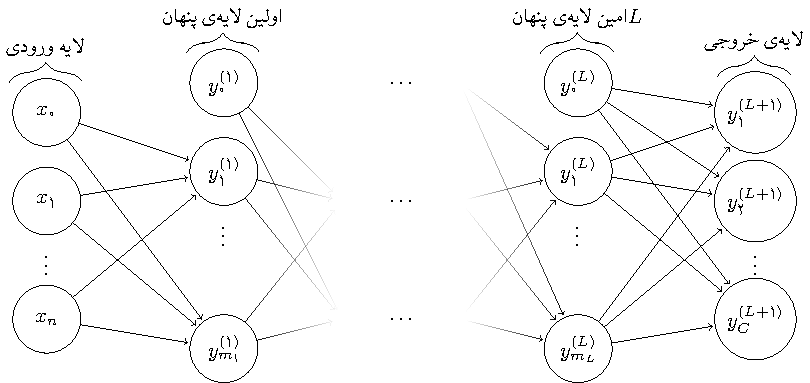
\includegraphics[width=.8\linewidth]{images/MLP}
			\caption{شبکه عصبی پرسپترون چند لایه}
			\label{fig:MLP}
%    \end{minipage}
\end{figure}
\subsection{روال آموزش پرسپترون}\label{sec:learning}
مجموعه‌ی آموزشی، متشکل از
$N$
زوج از الگوهای
$\{ ({\mathbf{x}}_i,{y}_i),\;i=1,\cdots,N\}$
است که در آن
$\mathbf{x}_i\in \mathbb{R}^n$
بردار نشان دهنده‌ی $i$امین ورودی و
$y_i\in \mathbb{R}$
طبقه‌ی درست متناظر با این نمونه است.
 اگر مسأله‌ی مدنظر، طبقه‌بندی نمونه‌ها به دو کلاس باشد، يعنی 
$y_i\in\{0,1\}$،
که در آن، صفر و یک برچسب دو کلاس هستند. %در حالت $K$ کلاسه

تابع هدف
\eqref{eq:missClassification}
را می‌توان در قالب مجموع مربعات خطا به صورت زیر نوشت که برای کمینه‌سازی مناسب‌تر است:
\begin{equation}
\frac{1}{2}\sum_{i=1}^N(y_i-\hat{y}_i)^2
\label{eq:SSE}
\end{equation}
اگر  $i$امین نمونه از داده‌ها به مدل داده شود، خروجی مدل به صورت
$\hat{y}_i = g(a_i) = g(\sum_{j=0}^n w_j x_j)$
خواهد بود. با جایگزینی
$\hat{y}_i$
در  تابع هدف
\eqref{eq:SSE}،
آن را می‌توان به صورت زیر برحسب
$w_i$
نوشت:
\begin{equation}
E(\mathbf{w}) = \frac{1}{2}\sum_{i}(y_i-\hat{y}_i)^2 = \frac{1}{2}\sum_{i}\left(y_i-g(\sum_{j=0}^n w_j x_j)\right)^2
\label{eq:cost_w}
\end{equation}
در این تابع خطا%
\LTRfootnote{Error Function}،‌
$x_j$
و
$y_i$
معلوم بوده و هدف، پیدا کردن وزن‌های بهینه
$(\mathbf{w})$
برای کمینه‌سازی خطاست.
پایه‌ی همه‌ی روش‌های مرسوم کمینه‌سازی در شبکه‌های عصبی الگوریتم
\textit{گرادیان کاهشی}
می‌باشد. در هر مرحله از یک روال تکراری، وزن‌های جدید بر اساس گرادیان تابع هدف، به صورت زیر بهنگام می‌شوند:
\begin{equation}
\mathbf{w}^{new} = \mathbf{w}^{old} - \eta\nabla E
\label{eq:delta_w}
\end{equation}
که
$\eta$
نرخ یادگیری و
$\nabla E$
گرادیان تابع خطاست. کافی است گرادیان تابع خطا برحسب وزن‌های اتصالات، محاسبه شده و وزن‌ها، مطابق رابطه‌ی بالا بروزرسانی شوند، که در ادامه بیان خواهد شد.
برای ساده‌سازی، خطای یک نمونه (بدون اندیس $i$)‌ را  درنظر بگیرید:
$$e =\frac{1}{2}(y-\hat{y})^2 $$
بنا به قاعده‌ی مشتق زنجیره‌ای داریم:
\begin{equation}\label{eq:partial_e}
      \frac{\partial e}{\partial w_{j}}
      =\frac{\partial e}{\partial y}\;
      \frac{\partial y}{\partial a}\;
      \frac{\partial a}{\partial w_{j}}
      =-(y-\hat{y})g'(a)x_j=(\hat{y}-y)g'(a)x_j
 \end{equation}
 لذا:
 \begin{align}\label{eq:partial_E}
\frac{\partial E}{\partial w_j} = \sum_i (\hat{y}_i-y_i)g'(a)x_j
\end{align}

بنابراین گرادیان تابع هزینه را به صورت زیر خواهیم داشت که می‌تواند در رابطه‌ی
\eqref{eq:delta_w}
برای بهنگام سازی وزن‌ها به‌کار گرفته شود:
\begin{equation}\label{eq:nabla_E}
\nabla E = \left[\frac{\partial E}{\partial w_0},\frac{\partial E}{\partial w_1},\dots,\frac{\partial E}{\partial w_n}\right]^T
\end{equation}
به عنوان مثال اگر 
$g(.)$
تابع همانی
$g(a)=a$
  باشد، مشتق آن بر حسب
  $a$
  یک شده و لذا روابط
  \eqref{eq:partial_e} 
  و
  \eqref{eq:nabla_E}   
برای نمونه‌ی $i$ام  به صورت زیر درخواهد آمد:
  \begin{equation}\label{eq:partial_e_gaa}
\frac{\partial e_i}{\partial w_{j}}
      =(\hat{y}_i-y)x_j
 \end{equation}
 که 
   \begin{equation}\label{eq:nabla_e_gaa}
\nabla e_i = \left[\frac{\partial e_i}{\partial w_0},\frac{\partial e_i}{\partial w_1},\dots,\frac{\partial e_i}{\partial w_n}\right]^T
 \end{equation}

 در رابطه‌ی 
 \eqref{eq:nabla_E}
 خطای همه‌ی داده‌های ورودی محاسبه می‌شود. اما به صورت معمول در روال آموزش شبکه‌های عصبی، خطای داده‌های آموزشی به صورت تکی یا گروهی در بروزرسانی وزن‌ها بکار برده می‌شوند:
 \begin{equation}
\mathbf{w}^{new} = \mathbf{w}^{old} - \eta\nabla e_i
\label{eq:delta_W_e}
\end{equation}
اگر 
$n=0$
و یا به عبارتی فقط یک داشته باشیم، رابطه‌ی فوق برای بهنگام کردن وزنها به صورت زیر درخواهد آمد (بدون اندیس مربوط به نمونه‌ی $i$ام):
 \begin{align}
w &= w - \eta\nabla e \nonumber\\
&= w - \eta(\hat{y}-y)\mathbf{x} \\
&= w + \eta(y-\hat{y})\mathbf{x}
\label{eq:delta_w_e}
\end{align}
با اندیس مربوط به نمونه‌ی $i$ام:
 \begin{align}
w &= w - \eta\nabla e_i \nonumber\\
&= w - \eta(\hat{y}_i-y_i)\mathbf{x}_i \\
&= w + \eta(y_i-\hat{y}_i)\mathbf{x}_i
\label{eq:delta_w_e_i}
\end{align}

$n$ 
هم تعداد ابعاد 
$\mathbf{x}$
را مشخص می‌کند و هم تعداد ابعاد
$\mathbf{w}$
را؛ لذا رابطه‌ی فوق می‌تواند با فرض برداری بودن 
$\mathbf{x}$
و
$\mathbf{w}$
به صورت زیر نوشته شود:
 \begin{equation}
\mathbf{w} = \mathbf{w} - \eta(\hat{y}_i-y_i)\mathbf{x}_i 
\label{eq:delta_W_x}
\end{equation}
%داریم:
%$\hat{y}_i = g(a_i) = \sum_{j=0}^n w_j x_j$



عنصر اصلی شبکه‌های چندلایه‌ی پرسپترونی%
\LTRfootnote{Multi Layer Perceptron (MLP)}
همین مدل پرسپترون ساده است. یک شبکه‌ی چند لایه معمولاً شامل یک لایه‌ی ورودی،‌ یک لایه‌ی خروجی و یک یا چند لایه‌ی پنهان است.
شکل
~\ref{fig:MLP}، 
یک نمونه شبکه عصبی چند لایه را نشان می‌دهد.
ساختار هر نود که با $y$‌ نشان داده شده است، همان ساختار مدل پرسپترون شکل
\ref{fig:perceptron}
است.
کلیات روش یادگیری در این شبکه‌ها
    و شبکه‌های پیچشی (شکل
\ref{fig:CNN})
که با نام
  \textbf{
  پس انتشار خطا}%
\LTRfootnote{ٍError Backpropagation}
\cite{Rumelhart:1988:LRB}
معروف است، مشابه روال فوق‌الذکر است.

\subsection{شبکه‌های عصبی پیچشی }
\label{sec:CNNs}
در شکل
~\ref{fig:CNN}، 
بخشی از یک شبکه‌ی پیچشی که با نام شبکه‌های پیچشی عمیق هم نامیده می‌شوند ملاحظه می‌شود. برخلاف شبکه‌های چندلایه‌ی پرسپترونی که ورودی در قالب بردار به شبکه داده می‌شود، ورودی شبکه‌های پیچشی یک تصویر است. اگر تصویر رنگی (مرکب از سه رنگ قرمز، سبز و آبی) باشد، مطابق شکل فوق‌الذکر، ورودی یک مکعب مستطیل خواهد بود.
در عموم شبکه‌های عصبی مرسوم، هر نود به همه نودهای لایه‌های مجاور متصل است، اما  در شبکه‌های عصبی پیچشی، هر نود فقط از تعدادی از نودهای لایه‌ی قبل تاثیر می‌پذیرد. این بخش کار، مشابه عمل پیچش (کانولوشن)‌ در پردازش سیگنال‌هاست که وجه تسمیه‌ی این شبکه‌ها به شبکه‌های عصبی پیچشی شده است.
همچنین برای نمایش‌ها نورون‌ها برخلاف روال معمول نمایش شبکه‌های پرسپترونی که نورون‌ها با دایره نمایش داده می‌شوند، در شبکه‌های پیچشی از مکعب استفاده می‌شود. مکعب خاکستری نمایش داده شده در شکل
~\ref{fig:CNN}
همان مدل پرسپترون نمایش داده شده در شکل
\ref{fig:perceptron}
است.  از آنجا که تعداد اتصالات در شبکه‌های پیچشی بسیار زیاد است، به صورت خط نمایش داده نمی‌شوند، بلکه گروهی از اتصالات دارای وزن‌، در قالب ماتریس یا مکعب مستطیل نمایش داده می‌شوند و یا اصلاً نمایش داده نشده و فقط تعداد آنها ذکر می‌شود
(شکل 
\ref{fig:vgg16}).

\begin{figure}[t]
\centering
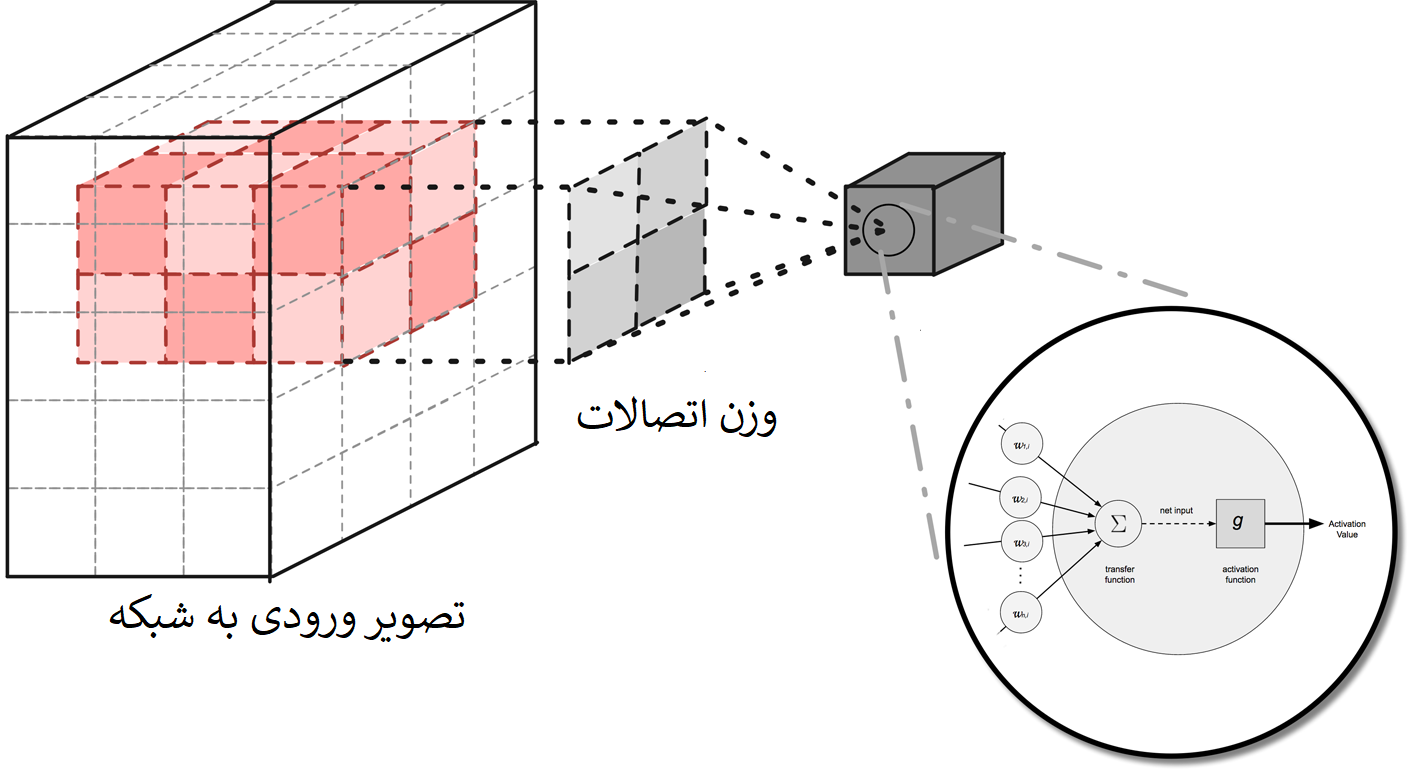
\includegraphics[width=.6\linewidth]{images/CNN1}
\caption{مدل شبکه‌ی عصبی پیچشی.
عموماً در نمایش شبکه‌های پیچشی از مکعب مستطیل برای نمایش نورون‌ها و از ماتریس (دوبعدی) یا مکعب مستطیل (سه‌بعدی) برای نمایش وزن‌ها استفاده می‌شود. مکعب خاکستری در واقع یک نورون با مدل پرسپترون نمایش داده شده در شکل
\ref{fig:perceptron}
است. اتصالات شبکه حکم فیلترهای یک شبکه‌ی پیچشی را دارند.
}
\label{fig:CNN}
\end{figure}



  از معروف‌ترین توپولوژی‌های ابداع شده از شبکه‌های پیچشی، مدل
\lr{VGG}
\cite{VGG_Simonyan15}
است که در
شکل
\ref{fig:vgg16}
معماری مدلی از آن با نام
\lr{VGG16}
نشان داده شد.
این مدل بیش از ۱۳۴ میلیون اتصال دارد. پنج گروه لایه‌ی پیچشی وظیفه‌ی استخراج ویژگی‌ها را دارند و سه لایه‌ی پرسپترونی آخر، کار طبقه‌بندی ویژگی‌های استخراج شده را انجام می‌دهند. این لایه‌ها در شکل
\ref{fig:vgg16}
به ترتیب با رنگ‌های زرد و بنفش مشخص شده‌اند. لایه‌های نارنجی رنگ بیانگر تابع فعالیت هستند و لایه‌های قرمز رنگ، لایه نمونه بردار یا انتخاب بیشینه %
\lr{(Max Pooling)}
%\LTRfootnote{Max Pooling}
نامیده می‌شوند که کار کوچک‌سازی تصویر را انجام داده و بدون وزن هستند. آخرین لایه به تعداد کلاس‌های مورد طبقه‌بندی، نورون دارد. در مدل اصلی آموزش دیده، هزار طبقه وجود دارد، اما برای کاربرد مدنظر این نوشتار، دو نورون خروجی برای دو دسته سبک نقاشی درنظر گرفته شده است.

جدول
\ref{tab:VGGModelParameters}
تعداد وزن‌های مدل شکل
\ref{fig:vgg16}
  را نشان می‌دهد.
ستون
\lr{Layer}
بیانگر نام لایه‌هاست که در شکل
\ref{fig:vgg16}
در ضلع زیرین مکعب مستطیل‌ها نوشته شده است.
ستون
\lr{Output Shape}
اندازه
خروجی هر لایه را نشان می‌دهد.
به عنوان نمونه، خروجی اولین لایه‌ی پیچشی (اولین لایه زرد رنگ شکل
\ref{fig:vgg16})
در اولین سطر جدول
\ref{tab:VGGModelParameters}
به صورت
$[\mathbf{64}, 224, 224]$
بیانگر آن است که ۶۴ فیلتر بر روی تصویر ورودی -- که در اینجا
$224\times224$
 بوده است -- اعمال شده و خروجی هر کدام یک تصویر
$224\times224$
می‌باشد.
ستون آخر، تعداد پارامترهای هر لایه را نشان می‌دهد.
برای اولین سطر،
اگر مشابه با شکل
~\ref{fig:CNN}،
اندازه هر فیلتر
$3\times3$
  درنظر گرفته شود، هر فیلتر برای یک تصویر رنگی
$3\times3\times3=27$
وزن اتصالی دارد که با احتساب بایاس ۲۸ وزن خواهد شد. لذا برای اولین لایه که ۶۴ فیلتر داریم، به تعداد
$64\times28=1792$
پارامتر خواهیم داشت%
\footnote{
هدف این نوشتار بیان تفصیلی شبکه‌های پیچشی نیست و به همین مقدار بسنده می‌شود.
برای آشنایی بیشتر با مدل‌های شبکه‌های عصبی پیچشی و چگونگی محاسبه تعداد پارامترهای آنها، مطالعه‌ی کتاب «یادگیری عمیق با پایتون»
\cite{franoischollet2017learning}
پیشنهاد می‌شود.
}.
چون تصویر مربعی درنظر گرفته شده است،
فقط در کنار ضلع پایین مربع‌های شکل
\ref{fig:vgg16}
اندازه‌ی آنها نوشته شده است.
  لایه‌هایی که بدون وزن بوده‌اند نمایش داده نشده‌اند؛ به همین دلیل شماره لایه‌ها پی‌درپی نیست.
تعداد پارامترها در اینجا همان تعداد اتصالات است که هر یک دارای یک وزن هستند
همان‌‌گونه که ملاحظه می‌شود این مدل بیش از ۱۳۰ میلیون اتصال دارد.
روال کلی آموزش شبکه،‌ همان روشی است که در بخش
\ref{sec:learning}
توضیح داده شد.
صرفنظر از برخی ظرافت‌ها و پیچیدگی‌های پیاده‌سازی عملی، یک مسئله مهم در مورد این شبکه‌ها زمان‌بر بودن آموزش آنهاست. با هر داده آموزشی (یا گروهی از داده‌ها) که به شبکه داده می‌شود، همه‌ی وزن‌ اتصالات باید بهنگام شوند. استفاده از کارت‌های گرافیکی با توان پردازشی بالای موازی امکان انجام چنین حجم زیادی از پردازش‌ها را مهیا کرده است؛
با این حال، کاهش حجم مدل، موجب کاهش میزان محاسبات و کمتر شدن حافظه‌ی مورد نیاز خواهد شد.
%

%  که همان‌گونه که ملاحظه می‌شود در آخر، لایه‌های تمام متصل وجود دارد. ابتدا ۵ لایه‌ی پیچشی (هر یک شامل چند لایه‌ی پیچشی و یک لایه‌ی نمونه‌بردار یا انتخاب بیشینه%
%\LTRfootnote{MaxPooling})
%وجود دارد که وظیفه‌ی استخراج ویژگی را به عهده دارند.
%خروجی آخرین لایه‌ی نمونه‌بردار به عنوان ویژگی‌های ورودی یک طبقه‌بند از نوع شبکه‌های عصبی چند لایه درنظر گرفته می‌شوند.
%این شبکه یک لایه‌ی ورودی ۴۰۹۶تایی دارد که در شکل
%\ref{fig:vgg16}
%با عنوان
%\lr{FC1}
%یک لایه کاملاً متصل (به لایه بعدی خود) است. این لایه در معماری‌های معمول با نام لایه مسطح%
%\LTRfootnote{Flatten}
%نامیده می‌شود.
%سپس لایه پنهان شبکه عصبی با ۴۰۹۶ نورون را شاهدیم و در انتها لایه‌ی چگال%
%\LTRfootnote{Dense}
%آخر را داریم که به تعداد کلاس‌ها نورون داشته و از نوع بیشینه‌ی نرم%
%\LTRfootnote{SoftMax}
%است.


\begin{table}[t]
\caption{
خلاصه مدل و پارامترهای مدل
\lr{VGG16}
نمایش داده شده در شکل
\ref{fig:vgg16}
برای یک تصویر ورودی فرضی با ابعاد
$224\times 224$.
این مدل
$134,268,738$
وزن دارد.
لایه‌هایی که بدون وزن بوده‌اند نمایش داده نشده‌اند.
اعداد پررنگ بیانگر تعداد فیلترهای (مجموعه‌ای از وزن‌ها) آن لایه است.
تعداد پارامترها ربطی به طول و عرض تصویر ورودی ندارد.
کاهش تعداد اتصالات (پارامترها) برای لایه‌های پیچشی بالای نقطه‌چین انجام خواهد شد.
}
\label{tab:VGGModelParameters}
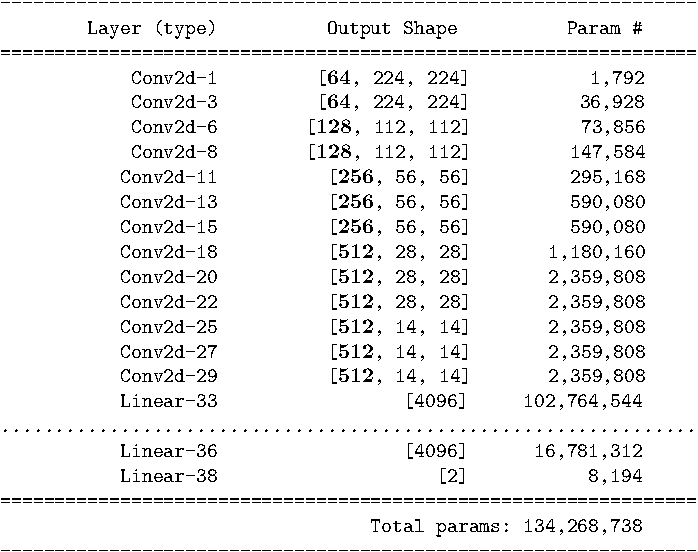
\includegraphics[width=.7\linewidth]{images/VGG16ModelParameters}
\end{table}


%\begin{figure}[t]
%\centering
%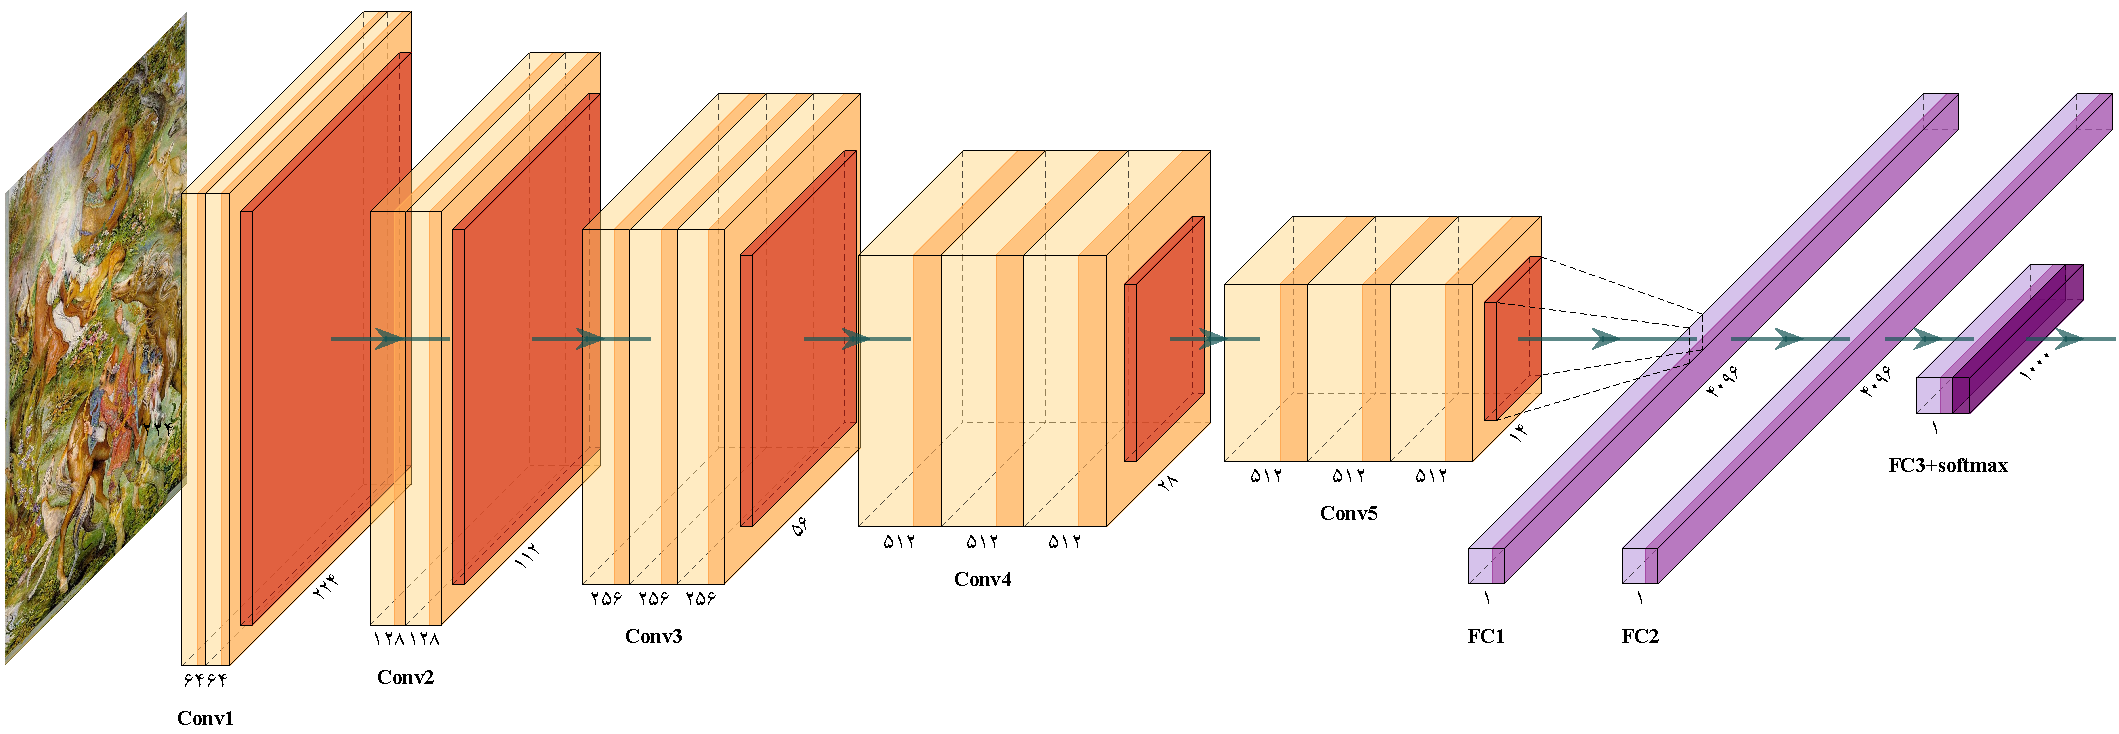
\includegraphics[width=1\linewidth]{images/vgg16-pruned.pdf}
%\caption{
%معماری مدل تبدیل شده‌ی تمام پیچشی. مدل پیچشی-چگال معادل این ساختار در شکل
%\ref{fig:FC}
%آمده است.
%}
%\label{fig:FConv}
%\end{figure}




\section{
کاهش حجم شبکه‌های عصبی پیچشی}
\label{sec:model_size_reduction}
هما‌گونه که در جدول
\ref{tab:VGGModelParameters}
 ملاحظه شد، مدلی مانند
\lr{VGG}
میلیون‌ها اتصال دارد. مدل اولیه بر روی 14 میلیون تصویر و برای طبقه‌بندی هزار موجودیت متفاوت آموزش دیده است. یکی از  مباحث حوزه یادگیری عمیق،
\textit{یادگیری انتقالی}%
\LTRfootnote{Transfer Learning}
است که هدف در آن به‌کارگیری یک مدل آموزش دیده در کاربردهای جدید است. به عنوان مثال اگر قرار باشد تصاویری متعلق به اشیاء جدیدی دسته‌بندی شوند که در هزار دسته‌ی اولیه‌ی
\lr{VGG}
نبوده‌اند، می‌توان با داشتن یک مدل آموزش دیده و فقط چند صد تصویر از اشیاء جدید، مدل قبلی را با صرف هزینه‌ی محاسباتی نسبتاً کم، دوباره آموزش داد تا  برای  شناسایی اشیاء جدید قابل استفاده باشد.
اگر مدل جدید فقط برای شناسایی چند دسته‌ی محدود موردنیاز باشد، احتمالاً بتوان بدون کاهش کارایی شبکه، تعدادی از اتصالات زائد%
\LTRfootnote{Redundant}
را حذف کرد.
این کاری است که به عنوان کاهش مدل انجام می‌شود.

\subsection{چالش‌ها}
\label{sec:Challenges}
راه حل اولیه‌ای که ممکن است به ذهن متبادر شود این است که به نوبت، هر یک از اتصالات حذف شده و تاثیر آن در کاهش خطای شبکه محاسبه شود.
اتصالاتی که حذف آنها مؤثر باشد،‌ هرس خواهند شد.
در پیاده‌سازی‌های معمول شبکه‌های پیچشی، امکان حذف یک اتصال به صورت مجزا فراهم نیست، اما می‌توان یک دسته از آنها (یک فیلتر یا یک لایه) را حذف کرد.
اگر قرار به حذف یک اتصال باشد،‌ به جای حذف آن، ضریب وزنی آن صفر قرار داده می‌شود.
به این ترتیب برای انتخاب فقط یک اتصال برای حذف، همه‌ی اتصالات به نوبت باید به صورت موقت حذف شده و
اتصالِ با کمترین تاثیر در کارایی شبکه، انتخاب و به صورت دائمی حذف شود.

روش فوق در عمل کارایی نخواهد داشت؛ عموماً به جای حذف تکی، انتخاب و حذف نورون‌ها به صورت گروهی انجام می‌شود؛
%مشابه این روال در  مغز انسان هم رخ می‌دهد. همه روزه
اما انتخاب و حذف وزن‌ها با این روش، یک مسئله‌ی بهینه‌سازی ترکیبیاتی است.
اگر در هر مرحله $k$‌ اتصال از بین $n$‌ اتصال انتخاب شوند،‌
$\binom{n}{k}$
حالت برای انتخاب وجود دارد.
% که اگر قرار به حذف
%$m\times k$
%اتصال باشد،‌ تعداد انتخاب‌ها
%$\binom{n}{k}$
%خواهد شد.
به عنوان نمونه اگر مدل شامل یک میلیون اتصال بوده و هدف، انتخاب و حذف  ده اتصال باشد،
$\binom{10^6}{10}\approx 2.75\times10^{53}$
حالت ممکن برای انتخاب این ده اتصال وجود دارد که بررسی همه آنها عملی نیست.

پس از حذف تعدادی از اتصالات، شبکه نیازمند آموزش مجدد است؛ که این عمل نیز زمان‌بر است.
اگر
شبکه شامل
$n$
اتصال باشد و در هر مرحله تعداد کمی از اتصالات هرس شوند،
بلافاصله نباید اقدام به انتخاب و حذف گروه بعدی اتصالات  نمود.
چون حذف  اتصالات قبلی، ساختار شبکه را مقداری تغییر داده است و شبکه برای یک مجموعه داده‌ی مشخص،‌ همان خروجی قبل از حذف  را تولید نمی‌کند. پس از هرس تعدادی از اتصالات، شبکه باید مجدداً مقداری آموزش داده شود تا اثر ناشی از حذف اتصالات جبران گردد.
% و سپس اقدام به انتخاب اتصالات بعدی گردد.
%این عملیات آموزش مجدد شبکه‌ زمان‌بر است.

ممکن است این پرسش مطرح شود که درصورت حذف تعدادی از اتصالات، وضعیت شبکه به چه صورت درخواهد آمد؟ همان‌گونه که پیش‌تر ذکر شد، عموماً در عمل، گروهی از اتصالات حذف می‌شوند. هر لایه در یک شبکه‌ی عصبی پیچشی، متضمن چندین فیلتر (گروهی از اتصالات) است. به عنوان نمونه،‌ اولین لایه‌ی مدل
\lr{VGG16}
مطابق جدول
\ref{tab:VGGModelParameters}
دارای ۶۴ فیلتر است.
حذف یک یا چند فیلتر از این لایه، خروجی و تعداد پارامترهای این لایه و ورودی به لایه‌ی بعدی را  تحت تاثیر قرار خواهد داد.
کاهش تعداد فیلترها، مترادف با کاهش حجم مدل است که هدف این نوشتار هم همین است.

%مقایسه حجم مدل
%\cite{SegNet2017}
%
%SegNet422.50488.7168031,052117DeepLab-LargeFOV [3]110.06160.7356181,99383FCN (learnt deconv) [2]317.09484.1197351,806539DeconvNet [4]474.65602.1597311,872877

%\subsection{استفاده از بسط تیلور در انتخاب وزن‌ها}\label{sec:Taylor}
همان‌گونه که در بخش
\ref{sec:CNNs}
 اشاره شد، بسیاری از مدل‌های پیچشی عمیق دارای تعداد بسیار زیادی نورون و اتصالات بین نورون‌ها می‌باشند.
%فرآیند انتخاب وزن‌هایی که از اهمیت کمتری در شبکه برخوردار هستند،‌ یک مسئله‌ی بهینه‌سازی ترکیبیاتی است.
حذف اتصالات زائد می‌تواند منجر به ایجاد مدلی کوچک‌تر شود که حجم حافظه و محاسبات کمتری نیاز داشته باشد.
مولچانوف و همکاران ایشان
شیوه‌ای مبتنی بر بسط تیلور تابع هدف
\eqref{eq:cost_w}
برای انتخاب وزن‌های زائد پیشنهاد داده‌اند
\cite{MolchanovTKAK17}
  که در این بخش این روش به صورت مبسوط بیان می‌شود.

\subsection{
استفاده از بسط تیلور در انتخاب وزن‌ها برای کاهش حجم مدل}
\label{sec:model_size_reduction_taylor}
فرض کنید
$\mathbf{w}$
بردار وزن‌های شبکه و
$E(\mathbf{w})$
تابع هزینه‌ی مسئله‌ی طبقه‌بندی باشد.
کاهش حجم مدل، به معنی کاستن تعداد درایه‌های
$\mathbf{w}$
است. برای بیان ریاضی مسئله، به جای حذف درایه‌ها، مؤلفه‌های مورد هرس از
$\mathbf{w}$
را صفر کرده و بردار جدید را
$\mathbf{W'}$
می‌نامیم. صفر شدن وزن یک اتصال مترادف با حذف  (هرس) ارتباط بین دو نود مربوطه است.
%وزن‌های جدید شبکه بعد از صفر کردن (هرس کردن) برخی از درایه‌های
%$\mathbf{w}$
%باشد.
% $i$امین درایه‌ی
%$\mathbf{w}$
%باشد.
%هرس
%$\mathbf{w}$
%باشد. در واقع
%$\mathbf{W'}$
%همان
%$\mathbf{w}$
%است که برخی از
%$w_i$ی
%آن صفر شده‌اند.
اگر فرض کنيم هيچ‌کدام از درايه‌های 
$\mathbf{w}$
برابر با صفر نباشد،
نرم صفر
$\mathbf{W'}$
$(\norm{\mathbf{W'}}_0)$،
تعداد مؤلفه‌های غیرصفر مدل، بعد از هرس را نشان می‌دهد.
%این فرض فقط به جهت بررسی
%\footnote{
%این فرض در پیاده‌سازی صادق خواهد بود. در هر دور از یک روال تکراری، مؤلفه‌های هرس شده، به واقع حذف شده و در ابتدای دور بعد
%}.
%برای سادگی
%$\mathbf{w}|_{w_i=0}$
%را با
%$\mathbf{W'}$
%نشان خواهیم داد.
به این ترتیب میزان تغییر خطای شبکه، ناشی از هرس کردن تعدادی از اتصالات آن را می‌توان به صورت
$|E(\mathbf{w})-E(\mathbf{W'})|$
نشان داد.
%اگر
%$\mathbf{w}$
%شامل هیچ درایه‌ی برابر با صفری نباشد،
%نرم صفر
%$\mathbf{W'}$
%مشخص‌کننده‌ی میزان کاهش تعداد وزن‌های مدل است.
% هر چقدر این مقدار
%کمتر باشد، فشردگی بیشتری خواهیم داشت.
فرض کنید میزان کاهشِ حجم نهایی مشخص است، یعنی به عنوان مثال برای
$B$
مفروض، مایل هستیم
$\norm{\mathbf{W'}}_0 \le B$.
کمتر بودن
$B$
معادل کمتر بودن مؤلفه‌های غیرصفر بردار وزن و به عبارت دیگر کمتر بودن اتصالات فعال مدل است. اگر اتصالاتِ دارای وزن برابر با صفر -- به عنوان اتصالات غیرفعال -- از بردار وزن حذف شوند، مدلی کوچک‌تر خواهیم داشت. حجم مدل جدید ناشی از هرس اتصالات، برابر با تعداد درایه‌های غیرصفر باقیمانده‌ (نرم صفر بردار) است.
%میزان کاهش حجم مدل متناسب با تعداد درایه‌هایی است...
با مفروضات فوق، مسئله‌ی کاهش تعداد اتصالات شبکه را می‌توان به صورت زیر نوشت:
\begin{equation}
\min_{\mathbf{W'}} |E(\mathbf{w})-E(\mathbf{W'})| \quad \mathtt{s.t.}\  \norm{\mathbf{W'}}_0 \le B
\label{eq:minEW}
\end{equation}


%$w_i$ی
%انتخاب شود که حذف (صفر) کردن آن کمترین تاثیر را بر روی تابع هزینه داشته باشد.
%اگر
%$E(\mathbf{w}|_{w_i=0})$
%بیانگر مقدار تابع هزینه، در حالتی باشد که وزن
%$w_i=0$
%آنگاه هدف مسئله به صورت زیر درخواهد آمد:
%
وقتی یک اتصال (وزن) حذف شود، میزان تغییر تابع خطا با استفاده از بسط تیلور تقریب زده می‌شود.
ابتدا مرور کوتاهی بر بسط تیلور داشته و سپس نحوه‌ی انتخاب اتصالاتی از شبکه که حذف آنها تاثیر کمی بر کارایی شبکه داشته باشد، بیان خواهد شد.

اگر تابع $f$‌در نقطه‌ی $a$ (نزدیک به $x$) بی‌نهایت بار مشتق‌پذیر باشد،‌ داریم:
\begin{align}
f(x) = \sum_{n=0} ^ {\infty} \frac {f^{(n)}(a)}{n!} (x-a)^{n}
= f(a)+\frac {f'(a)}{1!} (x-a)+ \frac{f''(a)}{2!} (x-a)^2+ \cdots %\nonumber
\end{align}
که در آن
$f^{(n)}(.)$
مشتق مرتبه $n$ام تابع $f(.)$ است.
اگر $f(.)$ یک تابع حقیقی مقدار چند متغیره باشد،‌ بسط تیلور آن به صورت زیر است:
\begin{align}
T(\mathbf{x}) = f(\mathbf{a}) + (\mathbf{x} - \mathbf{a})^\mathsf{T} \nabla f(\mathbf{a})%\nonumber\\
+ \frac{1}{2!} (\mathbf{x} - \mathbf{a})^\mathsf{T} \left \{\nabla^2 f(\mathbf{a}) \right \} (\mathbf{x} - \mathbf{a}) + \cdots
\end{align}
در حالت دو متغیره،‌ اگر از جملات مربوط به مشتقات دوم به بعد صرفنظر کنیم، داریم:
%بسط تیلور حالت دو متغیره را در نظر بگیرید:
\begin{align}
f(x,y) &\approx f(a,b) +\frac{\partial }{\partial x}f(a,b)(x-a)  + \frac{\partial }{\partial y}f(a,b) (y-b)
%\nonumber\\
%&+ \frac{1}{2!}\Big( (x-a)^2 f_{xx}(a,b) \nonumber\\
%&+ 2(x-a)(y-b) f_{xy}(a,b) +(y-b)^2 f_{yy}(a,b) \Big)
\end{align}
بسط فوق، فقط در راستای محور $x$ها حول نقطه‌ی
$(a,y)$
به صورت زیر است:
$$f(x,y) \approx f(a,y) + \frac{\partial }{\partial x}f(a,y)(x-a) $$
%+ \frac{1}{2}\frac{\partial^2}{\partial x^2}f(a,y)(x-a)^2$$
بر این اساس،‌ اگر به فرض، مدل شبکه عصبی دارای دو وزن
$w_1,w_2$
باشد،‌ تقریب خطی فوق  در راستای
$w_1$
حول نقطه‌ی
$(0,w_2)$
را به صورت خواهیم داشت:
\begin{equation}
\label{eq:E_w1_w2}
E(w_1,w_2) \approx E(0,w_2) + \frac{\partial}{\partial w_1}E(0,w_2)(w_1-0)
\end{equation}
پیش از این، بردار
$\mathbf{w}$
که تعدادی از درایه‌های آن صفر باشند، با
$\mathbf{W'}$
نمایش داده شد؛  برای حالت دو متغیره‌ی فوق‌الذکر و با فرض
$\mathbf{w}=[w_1,w_2]$
و
$\mathbf{W'}=[0,w_2]$،
رابطه‌ی
  \eqref{eq:E_w1_w2}
را می‌توان به صورت زیر نوشت:
\begin{equation}
E(\mathbf{w}) \approx E(\mathbf{W'}) + \frac{\partial}{\partial w_i}E(\mathbf{W'})(w_i-0),  \qquad i=1
\end{equation}
به عبارت دیگر در حالت کلی داریم:
\begin{equation}
E(\mathbf{w})-E(\mathbf{W'}) \approx  \frac{\partial}{\partial w_i}E(\mathbf{W'})w_i
\end{equation}
و لذا:
\begin{equation}
|E(\mathbf{w})-E(\mathbf{W'})| \approx  \left|\frac{\partial}{\partial w_i}E(\mathbf{W'})w_i\right|
\label{eq:equality}
\end{equation}
به این ترتیب مسئله‌ی کمینه‌سازی
\eqref{eq:minEW}
را می‌توان به صورت زیر نوشت:
\begin{equation}
\min \left|\frac{\partial}{\partial w_i}E(\mathbf{W'})w_i\right| \quad \mathtt{s.t.}\  \norm{\mathbf{W'}}_0 \le B
\label{eq:minREW}
\end{equation}
%صورت مسئله به فرم جدیدی درآمد، اما آنرا حل نخواهیم کرد!.
 هدف اصلی در هرس شبکه‌ها، یافتن اتصالاتی بود که حذف آنها کمترین تاثیر را بر کارایی شبکه داشته باشد.
 در رابطه‌ی
~\eqref{eq:equality}، 
مقدار
$|E(\mathbf{w})-E(\mathbf{W'})|$
بیانگر تغییر کارایی شبکه در صورت صفر شدن
$i$امین
مؤلفه‌ی
$\mathbf{w}$
است که با بسط تیلور،
معادل بودن تقریبی آن با
$\left|\frac{\partial}{\partial w_i}E(\mathbf{W'})w_i\right|$
نشان داده شد.
حال برای یافتن اتصالی که حذف آن
\textit{
  کمترین اثر در تغییر کارایی شبکه } را داشته باشد، کافی است آن
$w_i$
انتخاب شود که  کمترین مقدار
$\left|\frac{\partial}{\partial w_i}E(\mathbf{W'})w_i\right|$
را داشته باشد.
%  را خواهند داشت و می‌توانند کاندیدایی برای هرس باشند.
 محاسبه‌ی این عبارت فقط نیازمند وزن مربوطه و مشتق تابع هدف  است. ابزارهای مرسوم مورد استفاده در حوزه یادگیری عمیق
در روال تنظیم وزن‌ها، مقادیر وزن‌ها و مشتق تابع هدف را  در اختیار برنامه‌نویس قرار می‌دهند. %در شبکه‌های پیچشی
به آسانی%
\footnote{
البته این «به آسانی»، از آن به آسانی‌هاست که گاهی در منابع ریاضی ملاحظه می‌کنیم که «به آسانی نتیجه می‌شود
$\dots$».
مرتب‌سازی مشکلی ندارد، اما دسترسی به مشتق تابع در هر مرحله و صفر کردن وزن اتصالات، نیازمند ریزه‌کاری‌های فراوان برنامه‌نویسی است.
}
  می‌توان وزن‌ها را بر اساس حاصل‌ضرب مشتق تابع در وزن اتصال به صورت صعودی مرتب نموده و وزن با کمترین مقدار
 $\left|\frac{\partial}{\partial w_i}E(\mathbf{W'})w_i\right|$
   را انتخاب و حذف کرد.
در ادامه، کاربردی از این شیوه در مسئله‌ی تفکیک دو سبک نقاشی بیان خواهد شد.
%

\section{کاربرد در طبقه‌بندی نقاشی‌های سبک امپرسیونیسم و مینیاتور}\label{sec:results}
در این بخش در قالب یک کاربرد جدید، تاثیر هرس وزن‌ها بر پایه‌ی بسط تیلور را خواهیم دید.
روش مورد بررسی  در بستر پای‌تورچ%
\LTRfootnote{PyTorch: \url{https://pytorch.org/}}
  پیاده‌‌سازی شده است که به همراه تصاویر به‌کار برده شده، از گیت‌هاب نگارنده%
\LTRfootnote{\url{https://github.com/mamintoosi/CNN-pruning-using-Taylor-expansion}}
   قابل دسترس است.
کاربرد مدنظر، تفکیک تابلونگاره‌های دو سبک نقاشی مشهور است. فرض کنید چند صد تصویر از دو نوع سبک نقاشی --به عنوان تصاویر آموزشی-- و مدلی از قبل آموزش دیده%
\LTRfootnote{Pre-trained Model}
 بر روی اشیایی دیگر در دسترس است.
 یک مدل
\lr{VGG16}
حدود ۵۰۰ مگابایت حجم دارد.
 هدف، ایجاد یک مدل کم حجم‌تر
است که بتواند نقاشی‌های دیگری از این دو سبک که در مجموعه آموزشی نبوده‌اند را با دقت خوبی به دو دسته‌ی مربوطه کلاسه‌بندی نماید.
به این منظور دو سبک نقاشی امپرسیونیسم (برداشت‌گرایی) و مینیاتور با سبک فرشچیان انتخاب شدند.
در زمان نگارش این متن (شهریور ۹۹)
مسابقه‌ی تولید نقاشی با سبک برداشت‌گرایی مونه در کاگل%
\footnote{
سایت
\url{kaggle.com}
از معروف‌ترین سایت‌های برگزاری مسابقات یادگیری ماشین و داده‌کاوی است که جوایز  برخی از چالش‌های آن به چند ده هزار دلار هم می‌رسد.
}
  آغاز شده بود%
\LTRfootnote{Will you be the next Monet? \url{https://www.kaggle.com/c/gan-getting-started/}}.
هدف مسابقه‌ی مذکور ایجاد یک شبکه‌ی مولد رقابتی%
\LTRfootnote{Generative Adversarial Network}
  برای تولید خودکار نقاشی‌های جدید با سبک امپرسیونیسم کلود مونه%
\LTRfootnote{Claude Monet}
    بوده است.
 شیوه‌ی برداشت‌گرایی به عنوان سبکی از نقاشی توسط گروهی از هنرمندان ساکن پاریس آغاز شده است. نام این سبک از نام یک نقاشی از کلود مونه
  بنام
\textit{
    برداشت گرایی، طلوع خورشید}
(به فرانسوی:
\lr{Impression, soleil levant})
 گرفته شده‌اسـت%
\LTRfootnote{\url{https://en.wikipedia.org/wiki/Impressionism}}.
مسابقه‌ی فوق نقطه شروع ایده‌ی این کاربرد بود.
به عنوان سبک دیگری از نقاشی که یک سیستم تفکیک دو سبک  مدل‌سازی شود، مینیاتورهای (خُرد نگارگری‌های) محمود فرشچیان انتخاب شد.
شکل
~\ref{fig:MF-images}، 
دو نمونه از نقاشی‌های کلود مونه و فرشچیان را نشان می‌دهد.
تصویر فرضی ورودی به مدل
نمایش داده شده در شکل
\ref{fig:vgg16}،
مینیاتور
\textit{ضامن آهوی}
فرشچیان بوده است.


\begin{figure}[t]
\centering
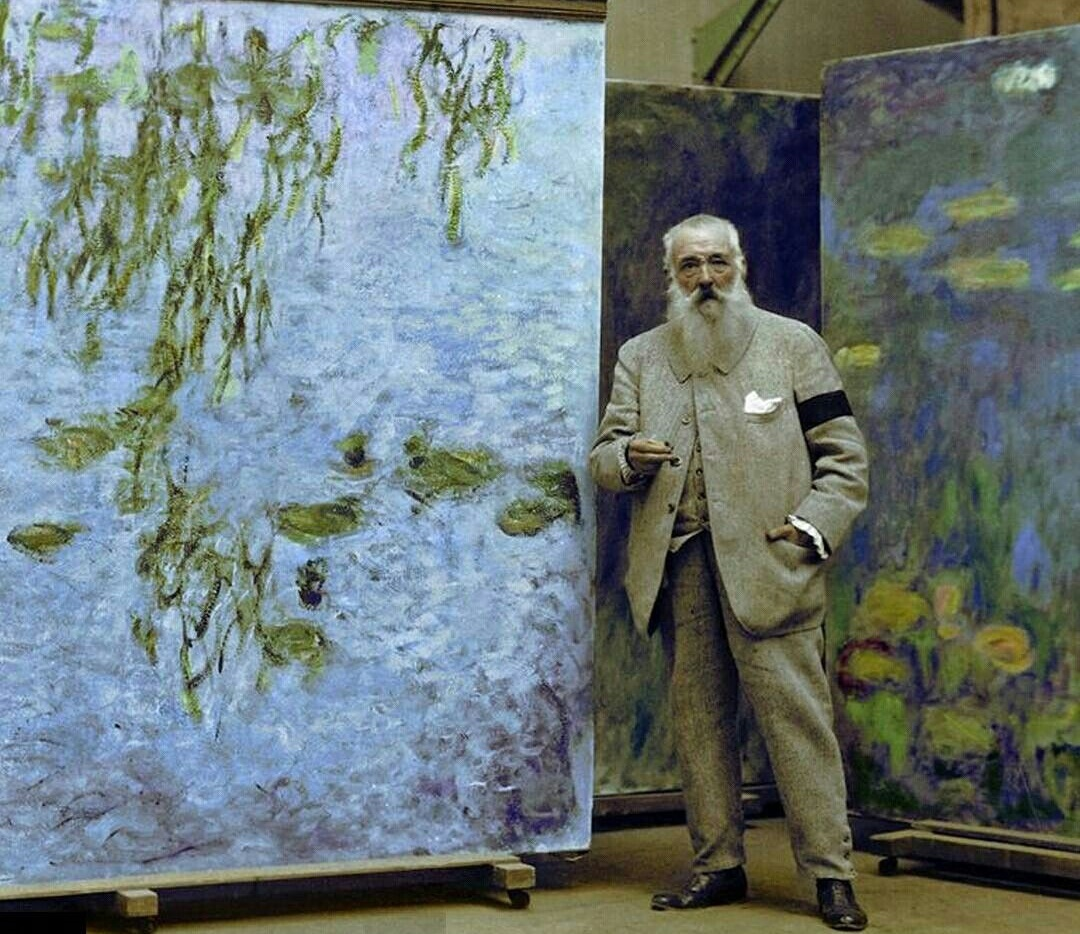
\includegraphics[width=.39\linewidth]{images/Claude-Monte.jpg}
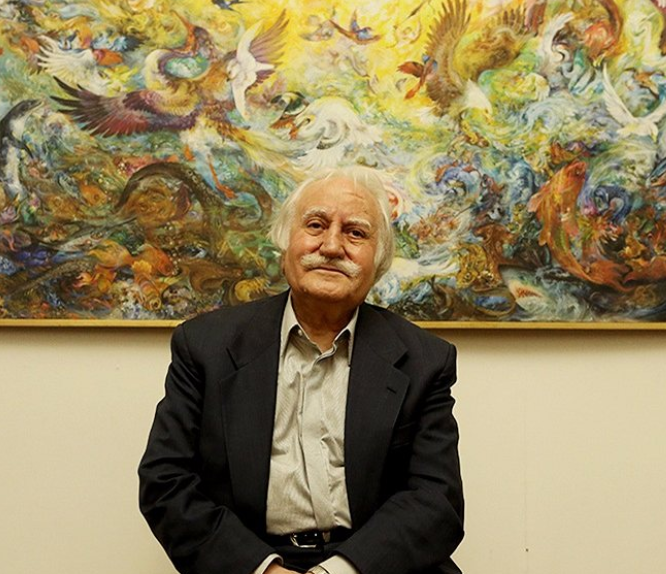
\includegraphics[width=.39\linewidth]{images/Mahmood-Farshchian.jpg}
\caption{
تصاویر کلود مونه (نقاش با سبک امپرسیونیسم) و محمود فرشچیان (مینیاتور) در کنار برخی از آثار ایشان.
}
\label{fig:MF-images}
\end{figure}

تا آنجا که نگارنده می‌داند هنوز کاری درخصوص طبقه‌بندی تابلونگاره‌های سبک‌های نقاشی انجام نشده است.
 البته
هدف از این نوشتار، ایجاد بهترین مدل برای طبقه‌بندی این سبک‌های نقاشی نیست؛
هدف اصلی آن است که نحوه‌ی استفاده از بسط تیلور در کاهش حجم مدل‌های یادگیری عمیق بیان شده و کاربرد جدیدی از آن بدینوسیله نشان داده شود.
لذا موضوع مقایسه با سایر روش‌های طبقه‌بندی مطرح نیست.

برای جمع‌آوری تصاویر موردنیاز، با یک خزنده‌ی وب%
\LTRfootnote{Web Crawler}، 
با جستجوی عبارات
«\lr{impressionism-claude-monet}»
 و «مینیاتور‌فرشچیان» در گوگل، حدود هزار تصویر برداشت شد.
%C:\gDrive\codes\Image-Crawler
با ملاحظه‌ی بصری، تعداد زیادی از نتایج نامطلوب حذف شدند
%\footnote{
%وجود مقداری کمی تصاویر نامرتبط در هر گروه مشکل خاصی ایجاد نمی‌کند.
%}
 و برای هر دسته ۳۱۳ تصویر نگه داشته شد.
%البته حذف تصاویر با کمی اغماض انجام شد. مثلاً تعداد معدودی از تصاویر شکسته نستعلیق به واقع جزو این خط محسوب نمی‌شدند اما از دیدگاه کلی شبیه به این خط بودند. برخی تابلوها دارای تصاویر پیس زمینه یا انسان هم بودند که اگر نوشته مربوطه بخش اصلی تصویر را تشکلیل می‌داد حذف نشدند.
%نمونه‌هایی از تصاویر باقیمانده در شکل
%\ref{fig:trainImages}
%قابل مشاهده هستند. حجم کل تصاویر
%$7.5$
% مگابایت است.
تصاویر به دو دسته‌ی آموزش و آزمون تقسیم شدند.
از مجموع ۶۲۶ تصویر، ۹۰درصد (۵۲۶ تصویر) به عنوان آموزش و ۶۲ تصویر باقیمانده  به عنوان داده آزمون درنظر گرفته شدند.
اندازه تصاویر ورودی کوچک و در حدود
$150\times150$
پیکسل بوده است.

%روش کلی اجرا، به صورت انتها به انتها
%\LTRfootnote{end-to-end}
%بوده و به جز تبدیل از بازه‌ی
%$[0,255]$
%به بازه‌ی
%$[0,1]$
%و افزایش تعداد نمونه‌ها
%\LTRfootnote{Augmentation}
%پردازش دیگری روی داده‌ها صورت نپذیرفته است.
%حداکثر زاویه ۴۵ درجه و میزان کمی تغییر مقیاس و جابجایی در راستای محورها به عنوان پارامترهای افزایش نمونه درنظر گرفته شده بودند.
%برای تعیین تعداد اِپُک بهینه،
%با اندازه دسته‌ی%
%\LTRfootnote{Batch Size}
%برابر با ۳۲، صد تکرار%
%\LTRfootnote{Epoch}
%  روی داده‌ها انجام شده است.
%شکل‌های
%\ref{nem:acc100}
%و
%\ref{nem:loss100}
%مقادیر صحت%
%\LTRfootnote{Accuracy}
%و خطا%
%\LTRfootnote{Loss}
%را برای داده‌های آموزشی و اعتبارسنجی نشان می‌دهند.
%
%%یک نمونه تغییر شکل یافته را نشان می‌دهد.
%
%در داده‌های آموزشی با افزایش تعداد تکرار، صحت، زیاد و خطا (زیان) کم می‌شود. اما در داده‌های اعتبارسنجی، صحت در دامنه‌ی حدوداً
%$0.65$
%تا
%$0.8$
%در نوسان است.
%برای تعیین تعداد اپک بهینه که مدل دچار بیش‌برازش نشده باشد، تکرار متناظر با خطای کمینه روی داده‌های اعتبارسنجی انتخاب می‌شود.
%اما خطای داده‌های اعتبارسنجی فرم واضحی ندارد. شاید به دلیل نسبتاً کم بودن داده‌های آموزشی و اعتبارسنجی و همچنین متنوع بودن تصاویر شاهد نموداری اینچنینی هستیم. تصاویر جمع‌آوری شده بسیار متنوع هستند و به سختی می‌توان الگوهای مشخصی را در آنها یافت.
%نمودار سبزرنگ تخمین بصری روال کلی خطای  اعتبارسنجی را نشان می‌دهد. مطابق این نمودار، تعداد تکرار حدود ۵۰ مناسب به نظر می‌رسد.
%مدل مورد استفاده در ادامه این بخش، مدل با پنجاه تکرار است.


ابتدا مدل اصلی از قبل آموزش دیده‌ی
%\lr{VGG}
شکل
\ref{fig:vgg16}
با پارمترهای جدول
\ref{tab:VGGModelParameters}
بر روی داده‌های آموزشی مورد آموزش مجدد قرار گرفت.
برای ارزیابی کارایی مدل از معیار صحت%
\LTRfootnote{Accuracy}
استفاده شده است. «صحت» عبارت از نسبت تعداد نمونه‌هایی که به درستی طبقه‌بندی شده‌اند به کل داده‌های مورد بررسی است و به صورت عددی در بازه‌ی صفر تا یک و یا برحسب درصد بیان می‌شود.
میزان صحت مدل بدست آمده،   روی داده‌های آزمون ۹۲ درصد بوده است که به منزله‌ی شناسایی درست ۵۹ تصویر از ۶۴ تصویر تست (آزمون) بوده است.
مدت زمان کل آموزش مجدد مدل فوق با پانزده تکرار روی ۶۲۶ تصویر آموزشی یک دقیقه و شش ثانیه (۶۶ ثانیه) بوده است. برنامه‌ روی سرورهای گوگل و مجهز به کارت گرافیک تسلا اجرا شده است. مشخصات سیستم مورد استفاده در جدول
\ref{tab:colabSpec}
آمده است.

\begin{figure*}[t]
\centering

\includegraphics[width=1\linewidth]{images/output4.jpg}
\caption{
خروجی روی ده تصویر آزمون. تصویر اول از سطر دوم، متعلق به سبک مینیاتور بوده است که به اشتباه متعلق به سبک امپرسیونیسم شمرده شده است.
}
\label{fig:output}
\end{figure*}

%https://colab.research.google.com/drive/1GeCFKPz01l3ayXOM0zPmpTaNFBgFhvj5
\begin{table}
\caption{مشخصات سیستم گوگل کولب، مورد استفاده در آزمایش‌ها.}
\label{tab:colabSpec}
\begin{latin}
\begin{tabular}{cl}
\hline
CPU & Intel(R) Xeon(R) CPU @ 2.20GHz\\
GPU & Tesla P100-PCIE-16GB 3584 CUDA cores , 16GB vRAM\\
RAM & ~12.6 GB\\
\hline
\end{tabular}
\end{latin}
\end{table}

زمان اجرای مورد نیاز این برنامه روی یک دستگاه معمولی
\lr{(Core i5)}
  و بدون بهره‌بردن از توان کارت گرافیک، حدوداً پنجاه برابر زمان اجرا روی سیستم فوق است.
% If you close the browser, it will stop in 90 minutes. If you open the browser, it will stop in 12 hours.
پس از آموزش اولیه، هرس شبکه با روش بسط تیلور انجام شد. همان‌‌گونه که در بخش
\ref{sec:Challenges}
 اشاره شد، پس از حذف اتصالات، شبکه باید مورد آموزش مجدد قرار گیرد تا اثر ناشی از هرس اتصالات، ترمیم شده، سایر اتصالات بتوانند خودشان را با این ساختار جدید وفق دهند. روش آموزش، مبتنی بر همان روال آموزشی است که در بخش
 \ref{sec:learning}
  توضیح داده شد.
روال تکراری حذف تعدادی از اتصالات و آموزش مجدد شبکه ۱۳ دقیقه و ۴۵ ثانیه به طول انجامید (۸۲۵ ثانیه).
حدود ۸۳ درصد وزن‌های شبکه هرس شدند. میزان صحت مدل نهایی بدست آمده بر روی داده‌های آزمون ۹۶ درصد بوده است.
شکل
\ref{fig:output}، 
نتیجه‌ی اجرای برنامه‌ی پایتون نوشته شده روی ده تصویر آزمون را نشان می‌دهد. سطر اول، نمونه‌ نقاشی‌های با سبک امپرسیونیسم هستند که همگی به درستی تشخیص داده شده‌اند. سطر دوم نمونه‌های متعلق به مینیاتور فرشچیان هستند که اولی به اشتباه «امپرسیونیسم» برچسب خورده است.
این تشخیص نادرست توسط ماشین، نشان‌گر خطاهایی است که انسان هم ممکن است در تشخیص داشته باشد. یک تفاوت اصلی شبکه‌های عصبی پیچشی در یادگیری عمیق با سایر طبقه‌بندهای معمول مثل شبکه‌های عصبی چند لایه آن است که در شبکه‌های پیچشی، استخراج ویژگی توسط خود شبکه انجام می‌شود. برای آشنایی با بصری‌سازی لایه‌های میانی شبکه که عمل استخراج ویژگی‌ها را انجام می‌دهند، به مرجع
\cite{franoischollet2017learning}
مراجعه شود.

\begin{table}[t]
\caption{
خلاصه مدل و پارامترهای مدل هرس شده با استفاده از بسط تیلور.
هرس وزن‌ها فقط برای لایه‌های بالای نقطه‌چین در این جدول انجام شده است.
اتصالات این لایه‌ها نسبت به لایه‌های متناظر در جدول
\ref{tab:VGGModelParameters}
نزدیک به ۹۵ درصد کاهش پیدا کرده‌اند.
اگر تعداد کل پارامترهای مدل مدنظر باشد، نسبت تعداد پارامترهای این مدل به مدل اولیه
$0.17$
است که به منزله‌ی کاهش ۸۳ درصدی می‌باشد.
به این ترتیب مدل بسیار کوچکتری حاصل شده است که کارایی کمتری از مدل اولیه ندارد.
%نمایش داده شده در شکل
%\ref{fig:FConv}.
}
\label{tab:VGG-prunned-ModelParameters}
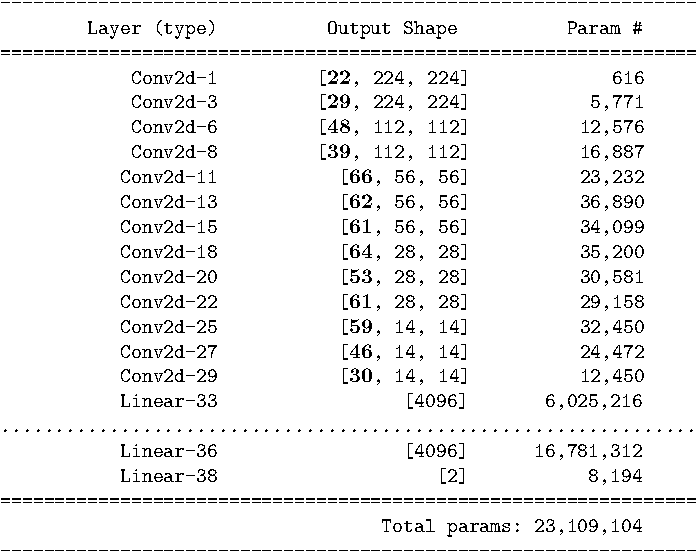
\includegraphics[width=.7\linewidth]{images/VGG16-prunned-ModelParameters}
\end{table}

جدول
\ref{tab:VGG-prunned-ModelParameters}، 
پارامترهای مدل
\lr{VGG16}
را بعد از اعمال کاهش تعداد وزن‌ها نشان می‌دهد.
در بالای نقطه‌چین جدول
~\ref{tab:VGGModelParameters}، 
به تعداد
$134,268,738-16,789,506 = 117,479,232$
پارامتر  داریم؛ این تعداد در جدول
~\ref{tab:VGG-prunned-ModelParameters}، 
به
$23,109,104-16,789,506 = 6,319,598$
رسیده است که بیانگر
نسبت
$6,319,598/117,479,232 = 0.05$
است. به عبارت دیگر، 
روش مورد بررسی، کاهش حدود ۹۵ درصدی تعداد اتصالات لایه‌ی پیچشی در مدل جدید نسبت به مدل اولیه را باعث شده است. البته اگر تمام اتصالات مدنظر قرار گیرد نسبت کاهش وزن‌ها ۸۳ درصد بوده است.
داده‌های این جدول و جدول
\ref{tab:VGGModelParameters}
 حاصل خروجی دستور
\lr{\texttt{summary}}
در پای‌تورچ
بر روی مدل هستند.
%\subsection{مقایسه‌ی زمان آزمون دو مدل}


\section{جمع‌بندی}
%نظریه تقریب یکی از نظریه‌های پرکاربرد ریاضی می‌باشد. یکی از روش‌های تقریب، استفاده از بسط تیلور است؛
نمایش کاربردهای ملموس نظریه‌های ریاضی می‌تواند برانگیزاننده‌ی اشتیاق دانش‌آموز یا دانشجو برای مطالعه و تعمق در آن حوزه باشد.
در نوشتار حاضر، کاربردی از بسط تیلور برای کوچک‌سازی یک مدل بزرگ شبکه‌های عصبی پیچشی به تفصیل شرح داده شد.
مبحث شبکه‌های عصبی پیچشی با شروع از مدل ساده پرسپترون و بر پایه‌ی دانش ریاضیات عمومی مرور گردید.
تابع هزینه‌ی شبکه‌های عصبی، میزان اختلاف خروجی شبکه با مقدار واقعی آن بر روی داده‌های آموزشی است.
روال آموزش، شامل مشتق‌گیری از تابع هدف و روش گرادیان کاهشی برای رسیدن به نقطه‌ی بهینه است.
در بسط تیلور، توابع از هر مرتبه مشتق‌پذیر را می‌توان به صورت چندجمله‌ای حول یک نقطه نمایش داد.
با بسط تیلور تابع هدف در نقطه‌ای که فقط یکی از وزن‌ها صفر است، و سنجش اختلاف مقدار این تابع با وضعیتی که همه وزن‌ها لحاظ شوند، رابطه‌ای برای برآورد اهمیت حضور هر اتصال شبکه بدست می‌آید. بر اساس این رابطه که حاصل‌ضرب وزن اتصال مورد هرس در مشتق تابع در آن نقطه است، اتصالاتی که تأثیر کمتری در کارایی شبکه دارند، شناسایی و حذف شدند.
کارایی شیوه‌ی مبتنی بر بسط تیلور در هرس اتصالات شبکه و کوچک کردن مدل بر روی کاربردی جدید (تفکیک تابلوهای با دو سبک نقاشی برداشت‌گرایی و مینیاتور) نشان داده شد.
در این کاربرد خاص،‌ تعداد پارامترهای مدل ۸۳ درصد کم شد و مدل جدیدی حاصل شد که گرچه فقط  ۱۷ درصد تعداد اتصالات مدل اولیه را دارد، اما همانند مدل اولیه دقت بالای ۹۲ درصد روی داده‌های تست را حفظ کرده است.

در این نوشتار فقط از تقریب مرتبه‌ی اول بسط تیلور استفاده شد. استفاده از تقریب‌های با مرتبه‌ی بالاتر می‌تواند از جمله کارهای آتی باشد. همچنین در این نوشتار، اهمیت همه‌ی اتصالات یکسان درنظر گرفته شده  و ملاک انتخاب اتصالات برای هرس، تنها حاصلضرب مقدار وزن اتصال در مشتق تابع هدف  بود که بر اساس بسط تیلور بدست آمده بود. اما ممکن است شرایط دیگری هم مدنظر باشد؛ به عنوان مثال، ممکن است کاربر ترجیح دهد به جای هرس شدن مختصر دو لایه‌ی پیچشی، کل یک لایه حذف شود.
تعیین حداکثر میزان فشردگی مدل، به شرط اینکه دقت کلی از میزان معینی کمتر نشود نیز می‌تواند از جمله موضوعات تحقیقاتی بعدی باشد.
%تلاش نگارنده بر آن بوده است که موضوع به صورت روان بیان شده و خواننده ضمن آشنایی با کاربردی از بسط تیلور،‌ با کلیات شبکه‌های عصبی پیچشی به عنوان یکی از ابزارهای اصلی حوزه‌ی یادگیری عمیق نیز آشنا شود.
%\clearpage
%گرچه که پیاده‌سازی این شیوه ممکن است خارج از


\section*{سپاس‌گزاری}
از داوران گرامی که با مطالعه‌ی دقیق و نظرات سازنده‌ی خود موجبات بهبود نوشتار حاضر را فراهم کردند، سپاس‌گزاری می‌کنم.

%\clearpage
%\newpage
{\small
%\onehalfspacing
\setlength{\itemsep}{-.5ex}
\bibliographystyle{ieeetr-fa}
\bibliography{MyReferences}
}

\noindent \rule{.4\linewidth}{0.8pt}\\
\noindent\footnotesize{\bfseries محمود امین‌طوسی } \\
\footnotesize{سبزوار، دانشگاه حکیم سبزواری، دانشکده ریاضی و علوم کامپیوتر }\\
\url{http://mamintoosi.ir},
\url{m.amintoosi@hsu.ac.ir}\\
\begin{tabular}{p{2 cm} p{14 cm} }
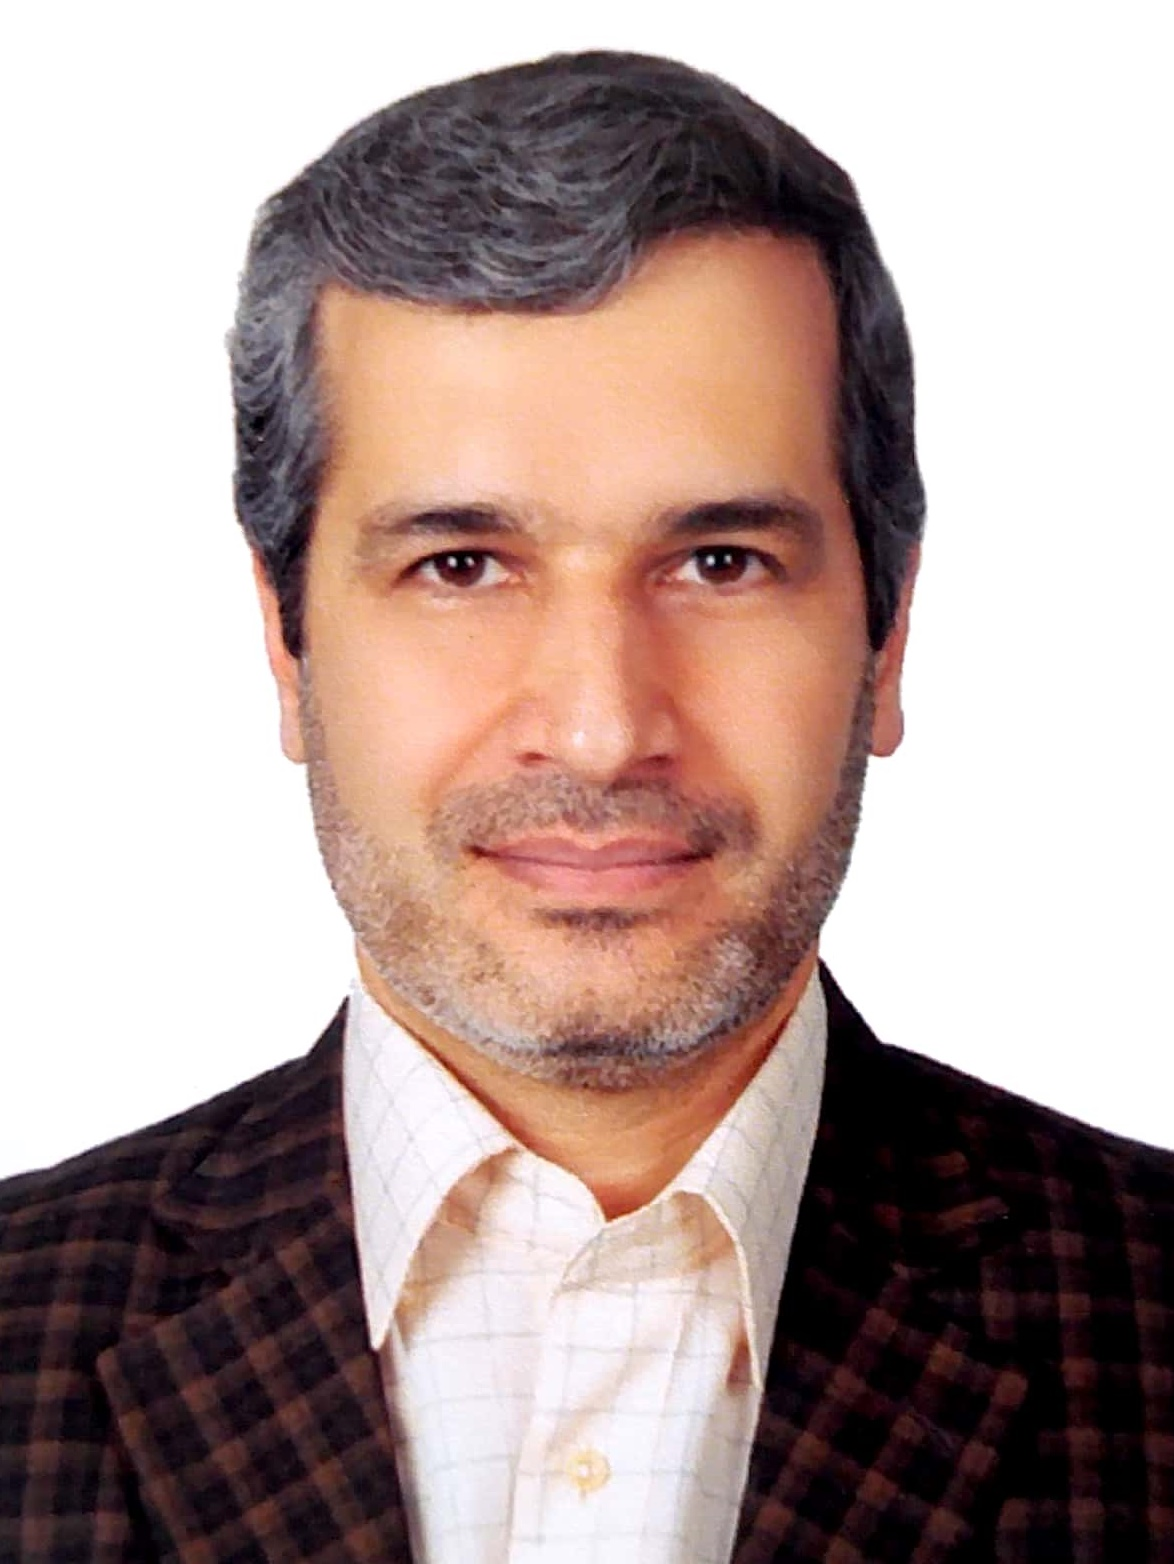
\includegraphics[width=18mm]{mAmintoosi1397.jpg}
&\vspace{-2.4cm}
\footnotesize
محمود امین‌طوسی، استادیار دانشگاه حکیم سبزواری است. وی دوره‌های کارشناسی و کارشناسی ارشد خود را در رشته‌های ریاضی (گرایش کاربرد در کامپیوتر) و  مهندسی کامپیوتر (گرایش نرم‌افزار) در  دانشگاه فردوسی به اتمام رسانده و دوره دکترای خود را در رشته مهندسی کامپیوتر (گرایش هوش مصنوعی) در دانشگاه علم و صنعت ایران گذرانده است.
علائق پژوهشی وی یادگیری ماشین، بینایی ماشین و بهینه‌سازی ترکیبیاتی می‌باشد. چاپ مقالات متعدد در کنفرانس‌ها و مجلات و انجام چند طرح تحقیقاتی از جمله کارهای پژوهشی وی می‌باشد.\\
\end{tabular}
\end{document} 